\chapter{Data Processing Examples}
\label{ch:examples}

\definecolor{lgray}{gray}{0.95}

This chapter showcases a variety of results that are possible when
processing different data sets with the Stereo Pipeline. It is also a
shortened guide that shows the commands used to process specific
mission data. There is no definitive method yet for making elevation
models as each stereo pair is unique. We hope that the following
sections serve as a cookbook for strategies that will get you started
in processing your own data. We recommend that you second check your
results against another source.

\section{Guidelines for Selecting Stereo Pairs}

When choosing image pairs to process, images that are taken with
similar viewing angles, lighting conditions, and significant surface
coverage overlap are best suited for creating terrain
models. Depending on the characteristics of the mission data set and
the individual images, the degree of acceptable variation will
differ. Significant differences between image characteristics
increases the likelihood of stereo matching error and artifacts, and
these errors will propagate through to the resulting data products.

Although images do not need to be map-projected before running the
\texttt{stereo} program, we recommend that you do run {\tt cam2map}
(or \texttt{cam2map4stereo.py})
beforehand, especially for image pairs that contain large topographic
variation (and therefore large disparity differences across the
scene, e.g., Valles Marineris).  Map-projection is especially necessary
when processing \ac{HiRISE} images. This removes the large disparity
differences between \ac{HiRISE} images and leaves only the small
detail for the Stereo Pipeline to compute. Remember that \ac{ISIS}
can work backwards through a map-projection when applying the camera
model, so the geometric integrity of your images will not be sacrificed
if you map-project first.

An alternative way of map-projection, that applies to non-ISIS imagery
as well, is with the \texttt{mapproject} tool (section
\ref{mapproj-example}).

Excessively noisy images will not correlate well, so images should be
photometrically calibrated in whatever fashion suits your purposes. If
there are photometric problems with the images, those photometric
defects can be misinterpreted as topography.

Remember, in order for \texttt{stereo} to process stereo pairs in
\ac{ISIS} cube format, the images must have had SPICE data associated
by running ISIS's \texttt{spiceinit} program run on them first.

%% \subsection{Comparing Examples to your System}

%% Since our first release we re-performed some of these examples and
%% recorded their processing time so you the user can judge how long it
%% will take you. Our examples were processed on our server called
%% `Lunokhod 2'. This server is a Dell PowerEdge Rack 900 purchased in
%% late 2009. Below are its specifications:

%% \begin{center}
%% \begin{tabular}{ l | l }
%% CPU & Dual E7420 Xeon at 2.13 GHz \emph{(16 logical cores)} \\ \hline
%% FSB & 1066 MHz \\ \hline
%% L2 Cache & 8 MB \\ \hline
%% Memory & 64 GB @ 667 MHz (mis-matched?) \\ \hline
%% Storage & Local RAID5 \\ \hline
%% OS & Red Hat Enterprise Linux 5.5 \\ \hline
%% BogoMIPS & 4256 \\ \hline
%% Color & Dell Graphite \\
%% \end{tabular}
%% \end{center}

%% The times recorded are listed in wall hours and CPU hours. Wall-hours
%% are how long it took the job to complete from the user's
%% perspective. CPU-hours are how much processing time it took to
%% complete. If the job took 30 wall-minutes on a 2 core system, it spent
%% 30 minutes in CPU 1 and CPU 2. Thus, the total CPU-hours would be
%% 1. This example, though correct, is not what always happens in the
%% real world. Inefficiency with managing multiple threads or the
%% complete lack of multithreaded code will bring wall hours up to CPU
%% hours. Your required CPU hours will vary based on CPU
%% architecture. Estimating your required CPU hours for your system can
%% be done by scaling with the BogoMIPS measurements. This can be read
%% from Linux systems with the command: \texttt{cat /proc/cpuinfo}

\section{Mars Reconnaissance Orbiter HiRISE}

\ac{HiRISE} is one of the most challenging cameras to use when making 3D
models because \ac{HiRISE} exposures can be several gigabytes each. Working
with this data requires patience as it will take time.

One important fact to know about HiRISE is that it is composed of
multiple linear CCDs that are arranged side by side with some vertical
offsets. These offsets mean that the CCDs will view some of the same
terrain but at a slightly different time and a slightly different
angle. Mosaicking the CCDs together to a single image is not a simple
process and involves living with some imperfections.

One cannot simply use the \ac{HiRISE} RDR products, as they do not
have the required geometric stability.  Instead, the \ac{HiRISE}
EDR products must be assembled using \ac{ISIS} \texttt{noproj}.
The USGS distributes a script in use by the \ac{HiRISE} team that
works forward from the team-produced `balance' cubes, which provides
a de-jittered, noproj'ed mosaic of a single observation, which is
perfectly suitable for use by the Stereo Pipeline (this script was
originally engineered to provide input for SOCET SET).  However,
the `balance' cubes are not available to the general public, and
so we include a program (\texttt{hiedr2mosaic.py}, written in
\href{http://www.python.org}{Python}) that will take \ac{PDS}
available \ac{HiRISE} EDR products and walk through the processing
steps required to provide good input images for \texttt{stereo}.

The program takes all the red CCDs and projects them using the \ac{ISIS}
{\tt noproj} command into the perspective of the RED5 CCD. From there,
{\tt hijitreg} is performed to work out the relative offsets between
CCDs. Finally the CCDs are mosaicked together using the average
offset listed from {\tt hijitreg} using the {\tt handmos} command,
and the mosaic is normalized with {\tt cubenorm}.
Below is an outline of the processing.

\begin{verbatim}
    hi2isis           # Import HiRISE IMG to Isis
    hical             # Calibrate
    histitch          # Assemble whole-CCD images from the channels
    spiceinit
    spicefit          # For good measure
    noproj            # Project all images into perspective of RED5
    hijitreg          # Work out alignment between CCDs
    handmos           # Mosaic to single file
    cubenorm          # Normalize the mosaic
\end{verbatim}

To use our script, first download a set of HiRISE data. Here is
an example, using wget to fetch all RED CCDs for a dataset and
process them.

\begin{verbatim}
  wget -r -l1 -np \
    "http://hirise-pds.lpl.arizona.edu/PDS/EDR/ESP/ORB_029400_029499/ESP_029421_2300/" \
    -A "*RED*IMG"
\end{verbatim}

Alternately, you can pass the \texttt{-\/-download-folder} option to
\texttt{hiedr2mosaic.py} and pass in the URL of the web page containing the EDR
files as the only positional argument.  This will cause the tool to first download
all of the RED CCD images to the specified folder and then continue with processing.

\begin{verbatim}
  hiedr2mosaic.py --download-folder hirise_example/ \
    http://hirise-pds.lpl.arizona.edu/PDS/EDR/ESP/ORB_029400_029499/ESP_029421_2300/
\end{verbatim}

Assuming you downloaded the files manually, go to the directory containing the files. You can run the
\texttt{hiedr2mosaic.py} program without any arguments to view a short
help statement, with the \texttt{-h} option to view a longer help statement,
or just run the program on the EDR files like so:

\begin{verbatim}
    hiedr2mosaic.py *.IMG
\end{verbatim}

If you have more than one observation's worth of EDRs in that
directory, then limit the program to just one observation's EDRs
at a time, e.g. \texttt{hiedr2mosaic.py PSP\_001513\_1655*IMG}.  If you
run into problems, try using the \texttt{-k} option to retain all of
the intermediary image files to help track down the issue.  The
\texttt{hiedr2mosaic.py} program will create a single mosaic file
with the extension \texttt{.mos\_hijitreged.norm.cub}.  Be warned that
the operations carried out by \texttt{hiedr2mosaic.py} can take many
hours to complete on the very large HiRISE images.

An example of using ASP with HiRISE data is included in the
\texttt{examples/HiRISE} directory (just type 'make' there).

\subsection{Columbia Hills}

%% \begin{tabular}{ l r c r c}
%% \textit{Prepping Files:}       & Wall Time & \texttt{+36:00:00.0} & CPU Time & \texttt{+36:00:00.0} \\
%% \textit{Processing in Stereo:} & Wall Time & \texttt{297:28:06.0} & CPU Time & \texttt{881:39:45.54} \\
%% \end{tabular}

\ac{HiRISE} observations
\href{http://hirise.lpl.arizona.edu/PSP_001513_1655}{PSP\_001513\_1655} and
\href{http://hirise.lpl.arizona.edu/PSP_001777_1650}{PSP\_001777\_1650}
are on the floor of Gusev Crater and cover the area where the \ac{MER}
Spirit landed and has roved, including the Columbia Hills.

\begin{figure}[h!]
\centering
  \subfigure[{\tt 3D Rendering}]{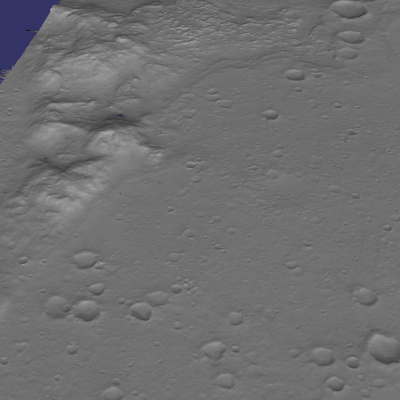
\includegraphics[width=3in]{images/examples/hirise/chills_hirise_example_400px.png}}
  \hfil
  \subfigure[{\tt KML Screenshot}]{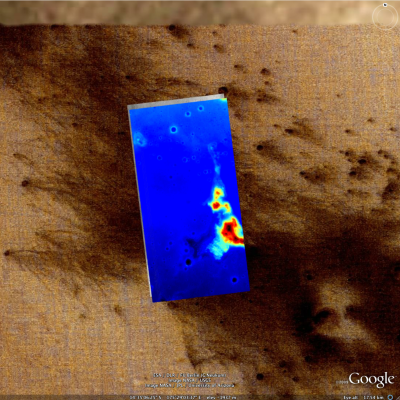
\includegraphics[width=3in]{images/examples/hirise/chills_hirise_ge_example_400px.png}}
\caption{Example output using HiRISE images PSP\_001513\_1655 and
  PSP\_001777\_1650 of the Columbia Hills.}
\label{fig:hirise_chills_example}
\end{figure}

\subsubsection*{Commands}

Download all 20 of the RED EDR \texttt{.IMG} files for each observation.
\begin{verbatim}
  ISIS 3> hiedr2mosaic.py PSP_001513_1655_RED*.IMG
  ISIS 3> hiedr2mosaic.py PSP_001777_1650_RED*.IMG
  ISIS 3> cam2map4stereo.py PSP_001777_1650_RED.mos_hijitreged.norm.cub \
                            PSP_001513_1655_RED.mos_hijitreged.norm.cub
  ISIS 3> stereo PSP_001513_1655.map.cub \
                 PSP_001777_1650.map.cub result/output
\end{verbatim}

\subsubsection*{stereo.default}

The stereo.default example file (appendix \ref{ch:stereodefault})
should apply well to HiRISE. Just set
\texttt{alignment-method} to \texttt{none} if
using map-projected imagery. If you are not using map-projected
imagery, set \texttt{alignment-method} to \texttt{homography} or
\texttt{affineepipolar}. The \texttt{corr-kernel} value can usually be
safely reduced to 21 pixels to resolve finer detail and faster
processing for images with good contrast.

\vfill

\section{Mars Reconnaissance Orbiter CTX}

\ac{CTX} is a moderate camera to work with. Processing times for
\ac{CTX} can be pretty long when using Bayes EM subpixel
refinement. Otherwise the disparity between images is relatively
small, allowing efficient computation and a reasonable processing time.

\subsection{North Terra Meridiani}

%% \begin{tabular}{l r c r c}
%% \textit{Processing in Stereo:} & Wall Time & \texttt{13:28:04.00} & CPU Time & \texttt{45:54:50.10} \\
%% \end{tabular}

In this example, we use map-projected images. Map-projecting the
images is the most reliable way to align the images for
correlation. However when possible, use non-map-projected images with
the \texttt{alignment-method affineepipolar} option. This greatly reduces
the time spent in triangulation. For all cases using linescan cameras,
triangulation of map-projected images is 10x slower than
non-map-projected images.

This example is distributed in the \texttt{examples/CTX} directory (type
'make' there to run it).

\begin{figure}[b!]
\centering
  \subfigure[{\tt 3D Rendering}]{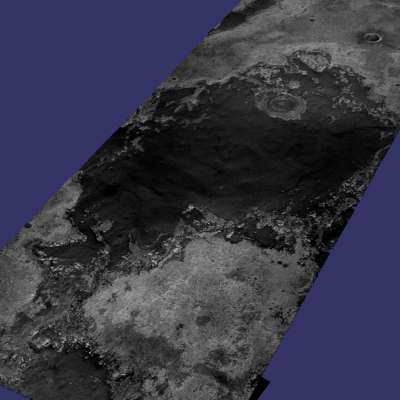
\includegraphics[width=3in]{images/examples/ctx/n_terra_meridiani_ctx_400px.png}}
  \hfil
  \subfigure[{\tt KML Screenshot}]{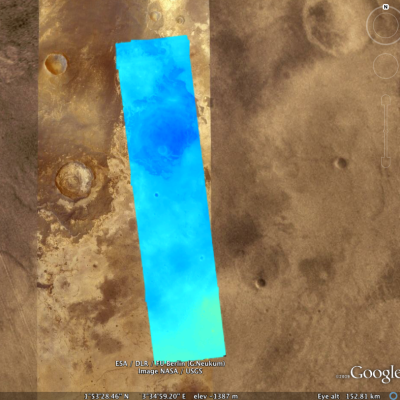
\includegraphics[width=3in]{images/examples/ctx/n_terra_meridiani_ctx_ge_400px.png}}
\caption{Example output possible with the CTX imager aboard MRO.}
\label{fig:ctx_example}
\end{figure}

\subsubsection*{Commands}

Download the \ac{CTX} images P02\_001981\_1823\_XI\_02N356W.IMG and
P03\_002258\_1817\_XI\_01N356W.IMG from the \ac{PDS}.
\begin{Verbatim}[commandchars=\\\{\}]
  ISIS 3> mroctx2isis from=P02_001981_1823_XI_02N356W.IMG to=P02_001981_1823.cub
  ISIS 3> mroctx2isis from=P03_002258_1817_XI_01N356W.IMG to=P03_002258_1817.cub
  ISIS 3> spiceinit from=P02_001981_1823.cub
  ISIS 3> spiceinit from=P03_002258_1817.cub
  ISIS 3> ctxcal from=P02_001981_1823.cub to=P02_001981_1823.cal.cub
  ISIS 3> ctxcal from=P03_002258_1817.cub to=P03_002258_1817.cal.cub
    \textnormal{you can also optionally run} ctxevenodd \textnormal{on the} cal.cub \textnormal{files, if needed}
  ISIS 3> cam2map4stereo.py P02_001981_1823.cal.cub P03_002258_1817.cal.cub
  ISIS 3> stereo P02_001981_1823.map.cub P03_002258_1817.map.cub results/out
\end{Verbatim}

\subsubsection*{stereo.default}

The stereo.default example file (appendix \ref{ch:stereodefault})
works generally well with all CTX pairs. Just set
\texttt{alignment-method} to \texttt{homography} or
\texttt{affineepipolar}.

\clearpage
\section{Mars Global Surveyor MOC-NA}

In the Stereo Pipeline Tutorial in Chapter~\ref{ch:moc_tutorial}, we
showed you how to process a narrow angle \ac{MOC} stereo pair that
covered a portion of Hrad Vallis. In this section we will show you
more examples, some of which exhibit a problem common to stereo
pairs from linescan imagers: ``spacecraft jitter'' is caused by
oscillations of the spacecraft due to the movement of other spacecraft
hardware.  All spacecraft wobble around to some degree but some are
particularly susceptible.

Jitter causes wave-like distortions along the track of the satellite
orbit in \acp{DEM} produced from linescan camera images.  This effect can
be very subtle or quite pronounced, so it is important to check your
data products carefully for any sign of this type of artifact. The
following examples will show the typical distortions created by this
problem.

Note that the science teams of \ac{HiRISE} and \ac{LROC} are actively
working on detecting and correctly modeling jitter in their respective
SPICE data. If they succeed in this, the distortions will still
be present in the raw imagery, but the jitter will no longer produce
ripple artifacts in the DEMs produced using ours or other stereo
reconstruction software.

\subsection{Ceraunius Tholus}

%% \begin{tabular}{l r c r c}
%% \textit{Prepping Files:}       & Wall Time & \texttt{00:02:42.30} & CPU Time & \texttt{00:02:42.06} \\
%% \textit{Processing in Stereo:} & Wall Time & \texttt{00:23:00.30} & CPU Time & \texttt{00:34:11.00} \\
%% \end{tabular}

Ceraunius Tholus is a volcano in northern Tharsis on Mars. It can
be found at 23.96 N and 262.60 E. This \ac{DEM} crosses the volcano's
caldera.

\begin{figure}[h]
\centering
  \subfigure[{\tt 3D Rendering}]{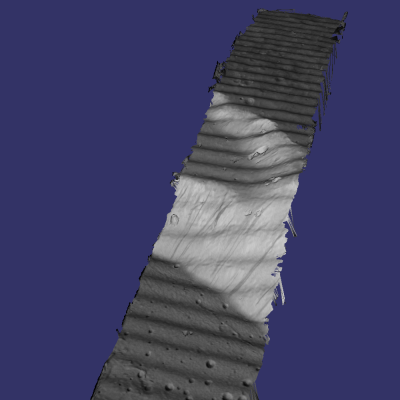
\includegraphics[width=3in]{images/examples/mocna/ceraunius_tholus_mocna_400px.png}}
  \hfil
  \subfigure[{\tt KML Screenshot}]{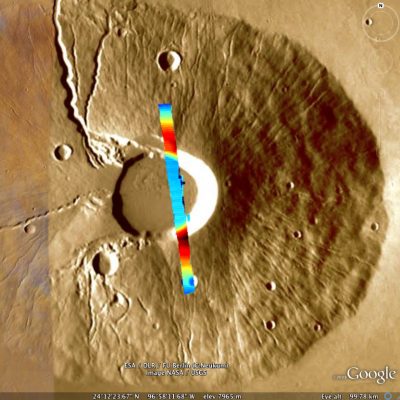
\includegraphics[width=3in]{images/examples/mocna/ceraunius_tholus_mocna_ge_400px.png}}
\caption{Example output for MOC-NA of Ceraunius Tholus. Notice the presence of severe washboarding artifacts due to spacecraft ``jitter.''}
\label{fig:mocna_ceraunius_example}
\end{figure}

\subsubsection*{Commands}

Download the M08/06047 and R07/01361 images from the \ac{PDS}.

\begin{verbatim}
  ISIS 3> moc2isis f=M0806047.img t=M0806047.cub
  ISIS 3> moc2isis f=R0701361.img t=R0701361.cub
  ISIS 3> spiceinit from=M0806047.cub
  ISIS 3> spiceinit from=R0701361.cub
  ISIS 3> cam2map4stereo.py M0806047.cub R0701361.cub
  ISIS 3> stereo M0806047.map.cub R0701361.map.cub result/output
\end{verbatim}

\subsubsection*{stereo.default}

The stereo.default example file (appendix \ref{ch:stereodefault}) works
generally well with all MOC-NA pairs. Just set \texttt{alignment-method}
to \texttt{none} when using map-projected imagery. If the images are not
map-projected, use \texttt{homography} or \texttt{affineepipolar}.

\section{Mars Exploration Rovers}\label{mer:example}

The Mars Exploration Rovers (MER) have several cameras on board
and they all seem to have a stereo pair. With ASP you are able to
process the PANCAM, NAVCAM, and HAZCAM camera imagery. ISIS has no
telemetry or camera intrinsic supports for these images. That however is
not a problem as their raw imagery contains the cameras' information in
JPL's CAHV, CAHVOR, and CHAVORE formats.

These cameras are all variations of a simple pinhole camera model so
they are processed with ASP in the \texttt{Pinhole} session instead of
the usual \texttt{ISIS}. ASP only supports creating of point
clouds. \emph{The *-PC.tif is a raw point cloud with the first 3
  channels being XYZ in the rover site's coordinate frame}. We don't
support the creation of DEMs from these images and that is left as an
exercise for the user.

An example of using ASP with MER data is included in the
\texttt{examples/MER} directory (just type 'make' there).

\subsection{PANCAM, NAVCAM, HAZCAM}

All of these cameras are processed the same way. We'll be showing 3D
processing of the front hazard cams. The only new things in the
pipeline is the new executable \texttt{mer2camera} along with the use
of \texttt{alignment-method epipolar}. This example is also provided
in the MER data example directory.

\begin{figure}[h!]
\centering
  \subfigure[{\tt Rectified Input}]{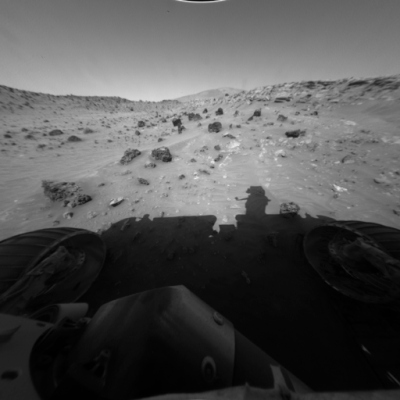
\includegraphics[width=3in]{images/examples/mer/fh01-L_sub_400px.png}}
  \hfil
  \subfigure[{\tt Output Point Cloud}]{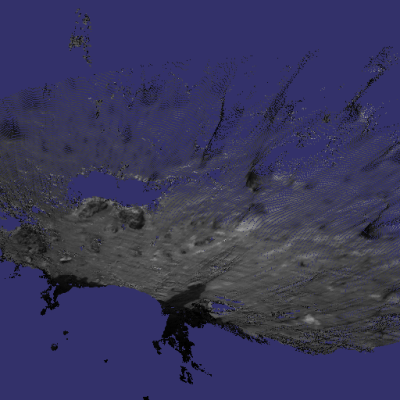
\includegraphics[width=3in]{images/examples/mer/fh01_pointcloud_400px.png}}
\caption{Example output possible with the front hazard cameras.}
\label{fig:mer_example}
\end{figure}

\pagebreak

\subsubsection*{Commands}

Download 2f194370083effap00p1214l0m1.img and
2f194370083effap00p1214r0m1.img from the \ac{PDS}.

\begin{verbatim}
  ISIS 3> mer2camera 2f194370083effap00p1214l0m1.img
  ISIS 3> mer2camera 2f194370083effap00p1214r0m1.img
  ISIS 3> stereo 2f194370083effap00p1214l0m1.img 2f194370083effap00p1214r0m1.img \
                 2f194370083effap00p1214l0m1.cahvore 2f194370083effap00p1214r0m1.cahvore \
                 fh01/fh01
\end{verbatim}

\subsection*{stereo.default}

The default stereo settings will work but change the following
options. The universe option filters out points that are not
triangulated well because they are too close \emph{robot's hardware}
or are extremely far away.

\begin{center}\begin{minipage}{5.5in}
\begin{Verbatim}[frame=single,fontsize=\small,label=additional settings for MER]
    alignment-method epipolar
    force-use-entire-range

    # This deletes points that are too far away
    # from the camera to truly triangulate.
    universe-center Camera
    near-universe-radius 0.7
    far-universe-radius 80.0
\end{Verbatim}
\end{minipage}\end{center}

\clearpage
\section{K10}\label{k10:example}

K10 is an Earth-based research rover within the Intelligent
Robotics Group at NASA Ames, the group ASP developers belong to. The
cameras on this rover use a simple Pinhole model. The use of ASP with
these cameras is illustrated in the \texttt{examples/K10} directory
(just type 'make' there).  Just as for the MER datatset (section
\ref{mer:example}), only the creation of a point cloud is supported.

\clearpage
\section{Lunar Reconnaissance Orbiter LROC NAC}
\label{lronac-example}

\subsection{Lee-Lincoln Scarp}

This stereo pair covers the Taurus-Littrow valley on the Moon where,
on December 11, 1972, the astronauts of Apollo 17 landed. However,
this stereo pair does not contain the landing site.  It is slightly
west; focusing on the Lee-Lincoln scarp that is on North Massif. The
scarp is an 80~m high feature that is the only visible sign of a deep
fault.

\begin{figure}[h!]
\centering
  \subfigure[{\tt 3D Rendering}]{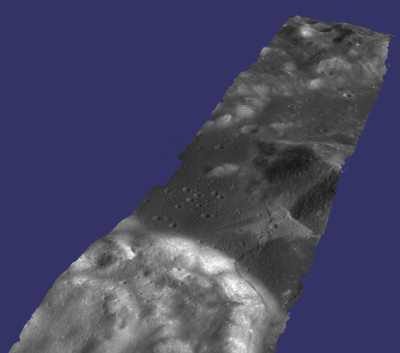
\includegraphics[width=3.8in]{images/examples/lrocna/lroc-na-example2_400px.png}}
  \hfil
  \subfigure[{\tt KML Screenshot}]{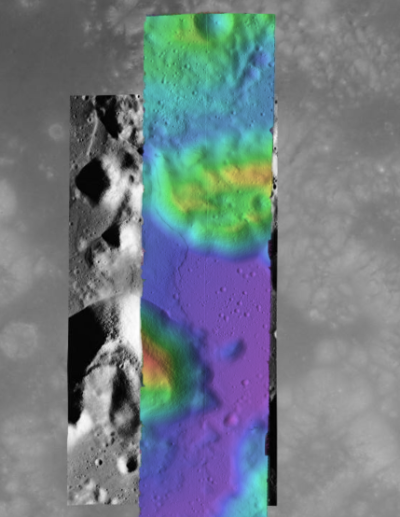
\includegraphics[width=3in]{images/examples/lrocna/lroc-na-ge_example2_400px.png}}
\caption{Example output possible with a LROC NA stereo pair, using both CCDs from each observation courtesy of the lronac2mosaic.py tool.}
\label{fig:lroc-na-example}
\end{figure}

\subsubsection*{Commands}

Download the EDRs for the left and right CCDs for observations
M104318871 and M104318871 from \url{http://wms.lroc.asu.edu/lroc/search}.
Alternatively you can search by original
IDs of 2DB8 and 4C86 in the PDS.

All ISIS preprocessing of the EDRs is performed via the
\texttt{lronac2mosaic.py} command. This runs \texttt{lronac2isis},
\texttt{lronaccal}, \texttt{lronacecho}, \texttt{spiceinit},
\texttt{noproj}, and \texttt{handmos} to create a stitched unprojected
image for a single observation. In this example we don't map-project
the images as ASP can usually get good results. More aggressive
terrain might require an additional \texttt{cam2map4stereo.py} step.

\begin{verbatim}
    ISIS 3> lronac2mosaic.py M104318871LE.img M104318871RE.img
    ISIS 3> lronac2mosaic.py M104311715LE.img M104311715RE.img
    ISIS 3> stereo M104318871LE*.mosaic.norm.cub M104311715LE*.mosaic.norm.cub \
              result/output --alignment-method affineepipolar
\end{verbatim}

\subsubsection*{stereo.default}

The defaults work generally well with LRO-NAC pairs, so you don't need
to provide a stereo.default file. Map-projecting is optional. When
map-projecting the images use \texttt{alignment-method none}, otherwise
use \texttt{alignment-method affineepipolar}. Better map-project results
can be achieved by projecting on a higher resolution elevation source
like the WAC DTM. This is achieved using the ISIS command \texttt{demprep}
and attaching to cube files via \texttt{spiceinit}'s SHAPE and MODEL
options.

\section{Apollo 15 Metric Camera Images}

\begin{tabular}{ r c r c}

\end{tabular}

Apollo Metric images were all taken at regular intervals, which means
that the same \texttt{stereo.default} can be used for all sequential
pairs of images. Apollo Metric images are ideal for stereo processing.
They produce consistent, excellent results.

The scans performed by ASU are sufficiently detailed to exhibit film
grain at the highest resolution.  The amount of noise at the full
resolution is not helpful for the correlator, so we recommend
subsampling the images by a factor of 4.

Currently the tools to ingest Apollo TIFFs into ISIS are not
available, but these images should soon be released into the PDS for
general public usage.

\subsection{Ansgarius C}

%% \begin{tabular}{ r c r c}
%% \multicolumn{3}{l}{ \emph{Prepping Files} } \\
%% Wall Time & \texttt{00:00:02.11} & CPU Time & \texttt{00:00:01.29} \\
%% \multicolumn{3}{l}{ \emph{Processing in Stereo} } \\
%% Wall Time & \texttt{01:52:23.00} & CPU Time & \texttt{21:36:07.61} \\
%% \end{tabular}

Ansgarius C is a small crater on the west edge of the far side of the
Moon near the equator. It is east of Kapteyn A and B.

\begin{figure}[h!]
\centering
  \subfigure[{\tt 3D Rendering}]{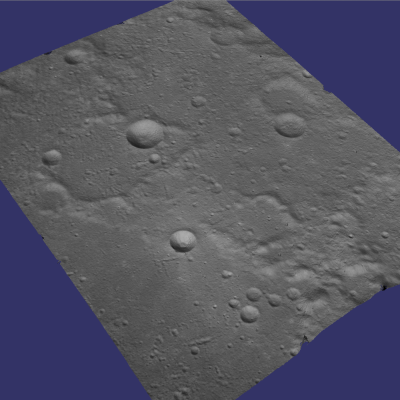
\includegraphics[width=3in]{images/examples/metric/metric_example_400px.png}}
  \hfil
  \subfigure[{\tt KML Screenshot}]{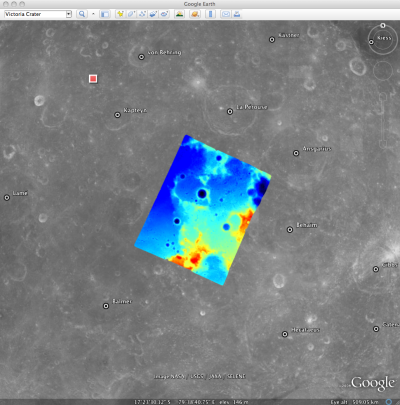
\includegraphics[width=3in]{images/examples/metric/metric_ge_example_400px.png}}
\caption{Example output possible with Apollo Metric frames AS15-M-2380 and AS15-M-2381.}
\label{fig:metric_example}
\end{figure}

\pagebreak

\subsubsection*{Commands}

Process Apollo TIFF files into \ac{ISIS}.
\begin{verbatim}
  ISIS 3> reduce from=AS15-M-2380.cub to=sub4-AS15-M-2380.cub sscale=4 lscale=4
  ISIS 3> reduce from=AS15-M-2381.cub to=sub4-AS15-M-2381.cub sscale=4 lscale=4
  ISIS 3> spiceinit from=sub4-AS15-M-2380.cub
  ISIS 3> spiceinit from=sub4-AS15-M-2381.cub
  ISIS 3> stereo sub4-AS15-M-2380.cub sub4-AS15-M-2381.cub result/output
\end{verbatim}

\subsubsection*{stereo.default}

The stereo.default example file (appendix \ref{ch:stereodefault})
works generally well with all Apollo pairs. Just set
\texttt{alignment-method} to \texttt{homography} or
\texttt{affineepipolar}.

%% \pagebreak


\section{Mars Express High Resolution Stereo Camera (HRSC)}

The HRSC camera on the Mars Express satellite is a complicated system,
consisting of multiple channels pointed in different directions plus
another super resolution channel.  The best option to create DEMs is to
use the two dedicated stereo channels.  These are pointed ahead of and
behind the nadir channel and collect a stereo observation in a single 
pass of the satellite.  Data can be downloaded from the Planetary Data
System (PDS) \url{http://pds-geosciences.wustl.edu/missions/mars_express/hrsc.htm}
or you can use the online graphical tool located at
\url{http://hrscview.fu-berlin.de/cgi-bin/ion-p?page=entry2.ion}.
Since each observation contains both stereo channels, one observation is sufficient 
to create a DEM.

HRSC data is organized into categories.  Level 2 is radiometrically corrected,
level 3 is corrected and map projected onto MOLA, and level 4 is corrected
and map projected on to a DEM created from the HRSC data.  You should use the
level 2 data for creating DEMs with ASP.  If you would like to download one
of the already created DEMs, it may be easiest to use the areoid referenced version
(.da4 extension) since that is consistent with MOLA.

What follows is an example for how to process HRSC data. One starts by fetching the two
stereo channels from:

\begin{verbatim}
http://pds-geosciences.wustl.edu/mex/mex-m-hrsc-3-rdr-v3/mexhrs_1001/data/1995/h1995_0000_s12.img
http://pds-geosciences.wustl.edu/mex/mex-m-hrsc-3-rdr-v3/mexhrs_1001/data/1995/h1995_0000_s22.img
\end{verbatim}

\subsubsection*{Commands}

You may need to download the HRSC kernel files in case using \texttt{web=true} with
\texttt{spiceinit} does not work.  You will also probably need to include the 
\texttt{ckpredicted=true} flag with \texttt{spiceinit}.  HRSC images are large
and may have compression artifacts so you should experiment on a small region
to make sure your stereo parameters are working well.  For this frame, the MGM
stereo algorithm performed better than block matching with subpixel mode 3.

\begin{verbatim}
  ISIS 3> hrsc2isis from=h1995_0000_s12.img to=h1995_0000_s12.cub
  ISIS 3> hrsc2isis from=h1995_0000_s22.img to=h1995_0000_s22.cub
  ISIS 3> spiceinit from=h1995_0000_s12.cub ckpredicted=true
  ISIS 3> spiceinit from=h1995_0000_s22.cub ckpredicted=true
  ISIS 3> stereo h1995_0000_s12.cub  h1995_0000_s22.cub \
           --stereo-algorithm 2 --cost-mode 3 mgm/out
\end{verbatim}

\begin{figure}[h!]
\centering
  \subfigure[{\tt Cropped input}]{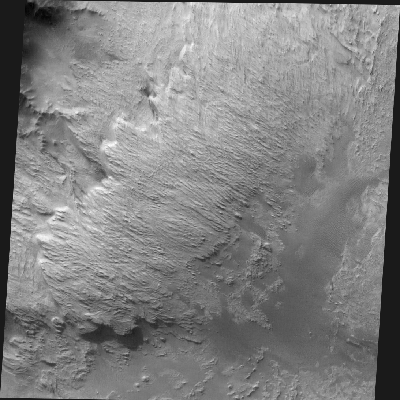
\includegraphics[width=2in]{images/examples/hrsc/hrsc_L.png}}
  \hfil
  \subfigure[{\tt Block matching with subpixel mode 3}]{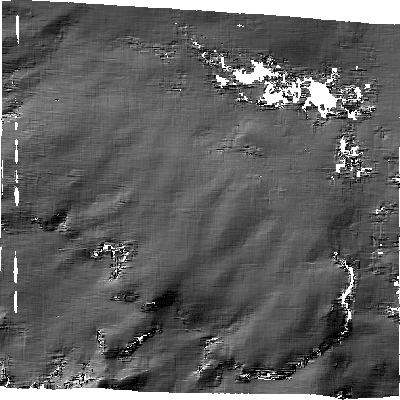
\includegraphics[width=2in]{images/examples/hrsc/hrsc_bm.png}}
  \hfil
  \subfigure[{\tt MGM algorithm with cost mode 3}]{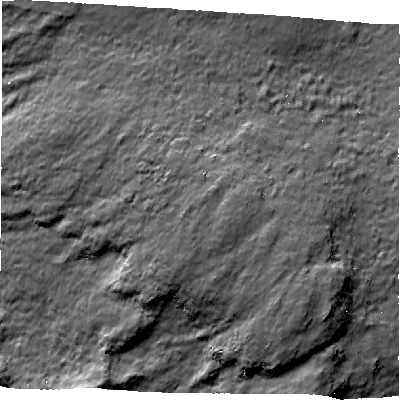
\includegraphics[width=2in]{images/examples/hrsc/hrsc_mgm.png}}
\caption{Sample outputs from a cropped region of HRSC frame 1995}
\label{fig:hrsc_example}
\end{figure}



%% \section{MESSENGER MDIS}

%% These results are a proof of concept showing off the strength of
%% building the Stereo Pipeline on top of \ac{ISIS}. Support for processing
%% MDIS stereo pairs was not a goal during our design of the software,
%% but the fact that an MDIS camera model exists in ISIS means that
%% it too can be processed by the Stereo Pipeline.

%% For future mappers, we suggest checking out Mercury Flyby 3 data which
%% was not available at the time of this writing. Flyby 3 and Flyby 2
%% seem to have covered some of the same terrain with the narrow angle
%% camera.

%% \subsection{Wide Angle on flyby 2}

%% In most flyby imagery it is very hard to find good stereo pairs.
%% This pair was taken from a single flyby just seconds apart. Note
%% also that this pair is taken from different wavelengths (the letter
%% at the end of the filename designates the current filter being used
%% on the wide angle camera). Unfortunately there is not enough of a
%% perspective change here to make anything other than the spherical
%% surface, but that alone is still an interesting result nonetheless.

%% \begin{figure}[h!]
%% \begin{minipage}{4in}
%% \includegraphics[width=4in]{images/examples/mdis/mdis_wide_example_400px.png}
%% \end{minipage}
%% \hfill
%% \begin{minipage}{2in}
%%   \caption{ A rough attempt at stereo reconstruction from MDIS imagery. }
%%   \label{fig:mdis_attempt}
%% \end{minipage}
%% \end{figure}

%% \subsubsection*{Commands}

%% \begin{verbatim}
%%   ISIS 3> mdis2isis from=EW0108825359A.IMG to=EW0108825359A.cub
%%   ISIS 3> mdis2isis from=EW0108825379C.IMG to=EW0108825379C.cub
%%   ISIS 3> spiceinit from=EW0108825359A.cub
%%   ISIS 3> spiceinit from=EW0108825359C.cub
%%   ISIS 3> mkdir result
%%   ISIS 3> stereo EW0108825359A.cub EW0108825379C.cub stereo/output
%% \end{verbatim}

%% \subsubsection*{stereo.default}

%% \begin{center}\begin{minipage}{5.5in}
%% \begin{Verbatim}[frame=single,fontsize=\small,label=stereo.default for MDIS]
%%     ### PREPROCESSING

%%     DO_INTERESTPOINT_ALIGNMENT 1
%%     INTERESTPOINT_ALIGNMENT_SUBSAMPLING 0
%%     DO_EPIPOLAR_ALIGNMENT 0

%%     FORCE_USE_ENTIRE_RANGE 0
%%     DO_INDIVIDUAL_NORMALIZATION 1

%%     PREPROCESSING_FILTER_MODE 2

%%     SLOG_KERNEL_WIDTH 1.5

%%     ### CORRELATION

%%     COST_BLUR 5
%%     COST_MODE 0

%%     H_KERNEL 25
%%     V_KERNEL 25

%%     H_CORR_MIN -10
%%     H_CORR_MAX 10
%%     V_CORR_MIN -2
%%     V_CORR_MAX 2

%%     SUBPIXEL_MODE 2

%%     SUBPIXEL_H_KERNEL 19
%%     SUBPIXEL_V_KERNEL 19

%%     ### FILTERING

%%     RM_H_HALF_KERN 5
%%     RM_V_HALF_KERN 5
%%     RM_MIN_MATCHES 60 # Units = percent
%%     RM_THRESHOLD 3
%%     RM_CLEANUP_PASSES 1

%%     FILL_HOLES 1

%%     ### DOTCLOUD

%%     NEAR_UNIVERSE_RADIUS 0.0
%%     FAR_UNIVERSE_RADIUS 0.0
%% \end{Verbatim}
%% \end{minipage}\end{center}

\clearpage

\section{Cassini ISS NAC}

This is a proof of concept showing the strength of building the Stereo
Pipeline on top of \ac{ISIS}.  Support for processing ISS NAC stereo pairs
was not a goal during our design of the software, but the fact that a
camera model exists in \ac{ISIS} means that it too can be processed by the
Stereo Pipeline.

Identifying stereo pairs from spacecraft that do not orbit their
target is a challenge. We have found that one usually has to settle
with images that are not ideal: different lighting, little perspective
change, and little or no stereo parallax. So far we have had little
success with Cassini's data, but nonetheless we provide this example
as a potential starting point.

\subsection{Rhea}

Rhea is the second largest moon of Saturn and is roughly a third the
size of our own Moon. This example shows, at the top right of both
images, a giant impact basin named Tirawa that is 220~miles across. The
bright white area south of Tirawa is ejecta from a new crater.  The
lack of texture in this area poses a challenge for our correlator. The
results are just barely useful: the Tirawa impact can barely be made
out in the 3D data while the new crater and ejecta become only noise.

\begin{figure}[p]
\centering
  \subfigure[{\tt Original Left Image}]{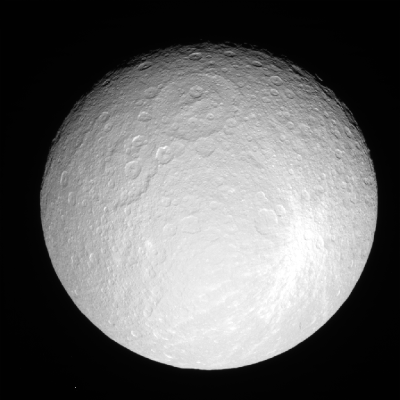
\includegraphics[width=3in]{images/examples/cassini/cassini_rhea_L_400px.png}}
  \hfil
  \subfigure[{\tt Original Right Image}]{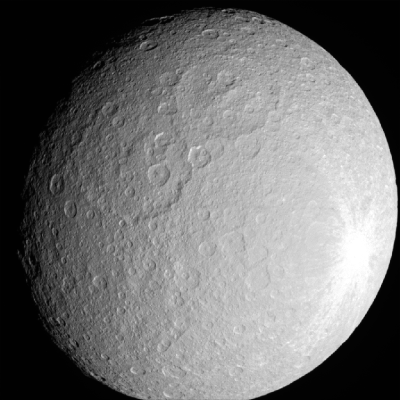
\includegraphics[width=3in]{images/examples/cassini/cassini_rhea_R_400px.png}}
  \\
  \subfigure[{\tt Map-Projected Left}]{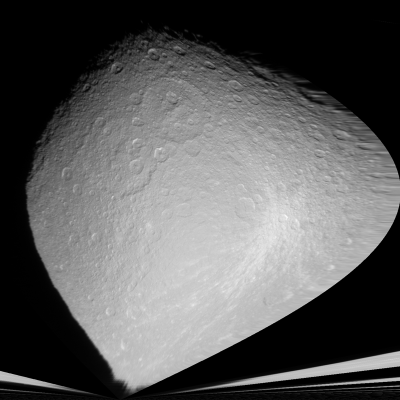
\includegraphics[width=3in]{images/examples/cassini/cassini_rhea_map_400px.png}}
  \hfil
  \subfigure[{\tt 3D Rendering}]{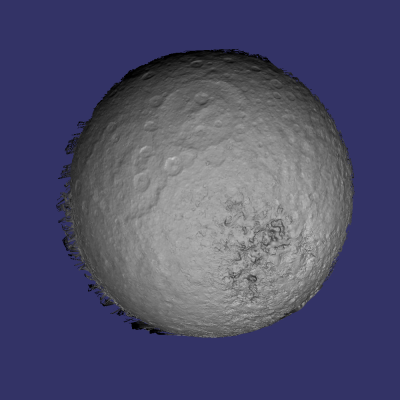
\includegraphics[width=3in]{images/examples/cassini/cassini_rhea_400px.png}}
\caption{Example output of what is possible with Cassini's ISS NAC}
\label{fig:cassini-exampe}
\end{figure}

\subsubsection*{Commands}

Download the N1511700120\_1.IMG and W1567133629\_1.IMG images and their label (.LBL) files from the \ac{PDS}.
\begin{verbatim}
  ISIS 3> ciss2isis f=N1511700120_1.LBL t=N1511700120_1.cub
  ISIS 3> ciss2isis f=W1567133629_1.LBL t=W1567133629_1.cub
  ISIS 3> cisscal from=N1511700120_1.cub to=N1511700120_1.lev1.cub
  ISIS 3> cisscal from=W1567133629_1.cub to=W1567133629_1.lev1.cub
  ISIS 3> fillgap from=W1567133629_1.lev1.cub to=W1567133629_1.fill.cub %Only one image
                                                                        %exhibits the problem
  ISIS 3> cubenorm from=N1511700120_1.lev1.cub to=N1511700120_1.norm.cub
  ISIS 3> cubenorm from=W1567133629_1.fill.cub to=W1567133629_1.norm.cub
  ISIS 3> spiceinit from=N1511700120_1.norm.cub
  ISIS 3> spiceinit from=W1567133629_1.norm.cub
  ISIS 3> cam2map from=N1511700120_1.norm.cub to=N1511700120_1.map.cub
  ISIS 3> cam2map from=W1567133629_1.norm.cub map=N1511700120_1.map.cub \
  ISIS 3>           to=W1567133629_1.map.cub matchmap=true
  ISIS 3> stereo N1511700120_1.map.equ.cub W1567133629_1.map.equ.cub result/rhea
\end{verbatim}

\subsubsection*{stereo.default}

\begin{center}\begin{minipage}{5.5in}
\begin{Verbatim}[frame=single,fontsize=\small,label=stereo.default for Cassini ISS]
    ### PREPROCESSING
    alignment-method none
    force-use-entire-range
    individually-normalize

    ### CORRELATION
    prefilter-mode 2
    prefilter-kernel-width 1.5

    cost-mode 2

    corr-kernel 25 25
    corr-search -55 -2 -5 10

    subpixel-mode 3
    subpixel-kernel 21 21

    ### FILTERING
    rm-half-kernel 5 5
    rm-min-matches 60 # Units = percent
    rm-threshold 3
    rm-cleanup-passes 1

\end{Verbatim}
\end{minipage}\end{center}

\section{Digital Globe Imagery}
\label{digital_globe_data}

Processing of Digital Globe images is described extensively in the
tutorial in chapter \ref{ch:dg_tutorial}.

\section{RPC Imagery, including GeoEye, Astrium, Cartosat-1, and PeruSat-1}
\label{rpc}

Some vendors, such as GeoEye with its Ikonos and two GeoEye satellites,
and Astrium, with its SPOT and Pleiades satellites, the Indian Cartosat-1 
satellite provide only
Rational Polynomial Camera (RPC) models. Digital Globe provides both
exact linescan camera models and their RPC approximations and ASP supports both. 
Apparently such is the case as well for PeruSat-1, but ASP supports only 
the RPC model for this satellite. 

RPC represents four 20-element polynomials that map geodetic coordinates
(longitude-latitude-height above datum)
to image pixels. Since they are easy to implement and fast to
evaluate, RPC represents a universal camera model providing a simple
approximation to complex exact camera models that are unique to each
vendor. The only downside is that it has less precision in our
opinion compared to the exact camera models.

In addition to supporting vendor-provided RPC models, ASP provides a
tool named \texttt{cam2rpc} (section \ref{cam2rpc}), that can be used to
create RPC camera models from ISIS and all other cameras that ASP
understands, including for non-Earth planets (currently only the Earth, Moon
and Mars are supported). In such situations, the planet datum must be
passed to the tools reading the RPC models, as shown below.

Our RPC read driver is GDAL. If the command \texttt{gdalinfo} can
identify the RPC information inside the headers of your image files (whether
that information is actually embedded in the images, or stored
separately in some auxiliary files with a convention GDAL understands),
ASP will likely be able to see it as well. This means that sometimes we
can get away with only providing a left and right image, with no extra
files containing camera information. This is specifically the case for
GeoEye, and Cartosat-1. Otherwise, the camera files must be specified
separately in XML files, as done for Digital Globe images (section
\ref{rawdg}) and PeruSat-1.

For a first test, you can download an example stereo pair from GeoEye's
website at \cite{geoeye:samples}. When we accessed the site, we
downloaded a GeoEye-1 image of Hobart, Australia. As previously stated
in the Digital Globe section, these types of images are not ideal for
ASP. This is both a forest and a urban area which makes correlation
difficult. ASP was designed more for modeling bare rock and ice. Any
results we produce in other environments is a bonus but is not our
objective.

\begin{figure}[h!]
\centering
  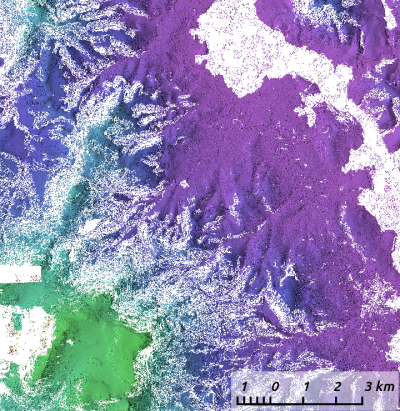
\includegraphics[width=2.0in]{images/examples/geoeye/GeoEye_ContextRender_400px.png}
  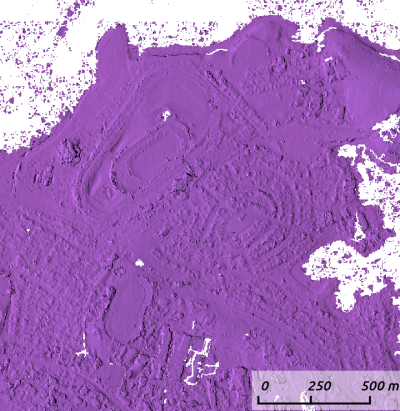
\includegraphics[width=2.0in]{images/examples/geoeye/GeoEye_CloseUp_400px.png}
  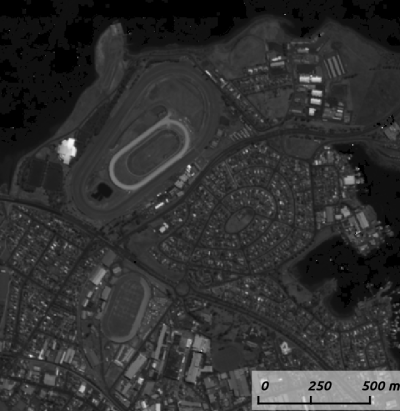
\includegraphics[width=2.0in]{images/examples/geoeye/GeoEye_CloseUpDRG_400px.png}
\caption{Example colorized height map and ortho image output.}
\label{fig:geoeye-nomap-example}
\end{figure}

\subsubsection*{Command}

\begin{verbatim}
   stereo -t rpc po_312012_pan_0000000.tif po_312012_pan_0010000.tif geoeye/geoeye
\end{verbatim}

(For Cartosat data sometimes one should overwrite the *RPC.TXT files that are present
with the ones that end in RPC\_ORG.TXT.)

If RPC cameras are specified separately, the \texttt{stereo} command
looks as follows. This example is for Mars, with the RPC models created
with \texttt{cam2rpc} from ISIS cubes.  So the datum has to be set.

\begin{verbatim}
  stereo -t rpc --datum D_MARS left.tif right.tif left.xml right.xml run/run
\end{verbatim}

For terrains having steep slopes, we recommend that images be
map-projected onto an existing DEM before running stereo. This is
described in section \ref{mapproj-example}. As above, if the cameras
are specified separately (as xml files), they should be on the command line,
otherwise they can be omitted.


If the RPC coefficients are
not stored in the original Tif images, but rather in associated .RPB or
\_RPC.TXT files, \texttt{mapproject} creates
these files automatically for each map-projected image.

\subsubsection*{stereo.default}

The stereo.default example file (appendix \ref{ch:stereodefault})
works generally well with all GeoEye pairs. Just set
\texttt{alignment-method} to \texttt{affineepipolar} or
\texttt{homography}.


\section{SPOT5 Imagery}
\label{sec:spot5}

SPOT5 is a CNES (Space Agency of France) satellite launched on May 2002 and 
decommissioned in March 2015.  SPOT5 contained two High Resolution Stereoscopic 
(HRS) instruments with a ground resolution of 5 meters.  These two cameras were
pointed forwards and backwards, allowing capture of a stereo image pair in
a single pass of the satellite.

ASP supports only images from the HRS sensors on SPOT5.  These images come in
two parts, the data file (extension \texttt{.bil} or \texttt{.tif}) and the header file
the data file (extension \texttt{.dim}).  The data file can be either a plain 
binary file with no header information or a GeoTIFF file.  The header file is a 
plain text XML file.  When using SPOT5 images with ASP tools, pass in the data file
as the image file and the header file as the camera model file.

All ASP tools can handle \texttt{.bil} images (and also \texttt{.bip}
and \texttt{.bsq}) as long as a similarly named \texttt{.dim} file
exists that can be looked up. The lookup succeeds if, for example, the
\texttt{.dim} and \texttt{.bil} files differ only by extension (lower or
upper case), or, as below, when an IMAGERY.BIL file has a corresponding
METADATA file.

You can find a sample SPOT5 image at 
\url{http://www.geo-airbusds.com/en/23-sample-imagery}.

One issue to watch out for is that SPOT5 data typically comes in a standard
directory structure where the image and header files always have the same name.
The header (camera model) files cannot be passed into the \texttt{bundle\_adjust} tool with the
same file name even if they are in different folders.  A simple workaround is to create
symbolic links to the original header files with different names:

\begin{verbatim}
    > ln -s  front/SEGMT01/METADATA.DIM front/SEGMT01/METADATA_FRONT.DIM
    > ln -s  back/SEGMT01/METADATA.DIM  back/SEGMT01/METADATA_BACK.DIM
    > bundle_adjust -t spot5 front/SEGMT01/IMAGERY.BIL back/SEGMT01/IMAGERY.BIL \
      front/SEGMT01/METADATA_FRONT.DIM back/SEGMT01/METADATA_BACK.DIM -o ba_run/out
    > stereo -t spot5 front/SEGMT01/IMAGERY.BIL back/SEGMT01/IMAGERY.BIL  \ 
      front/SEGMT01/METADATA_FRONT.DIM back/SEGMT01/METADATA_BACK.DIM \ 
      st_run/out --bundle-adjust-prefix ba_run/out
\end{verbatim}

You can also map project the SPOT5 images before they are passed to the 
\texttt{stereo} tool.  In order to do so, you must first use the 
\texttt{add\_spot\_rpc} tool to generate an RPC model approximation of
the SPOT5 sensor model, then use the \texttt{spot5maprpc} session type
when running stereo on the map projected images.

\begin{verbatim}
    > add_spot_rpc front/SEGMT01/METADATA.DIM -o front/SEGMT01/METADATA.DIM
    > add_spot_rpc back/SEGMT01/METADATA.DIM  -o back/SEGMT01/METADATA.DIM
    > mapproject sample_dem.tif front/SEGMT01/IMAGERY.BIL front/SEGMT01/METADATA.DIM 
      front_map_proj.tif -t rpc
    > mapproject sample_dem.tif back/SEGMT01/IMAGERY.BIL back/SEGMT01/METADATA.DIM 
      back_map_proj.tif -t rpc
    > stereo -t spot5maprpc front_map_proj.tif back_map_proj.tif  \ 
      front/SEGMT01/METADATA.DIM back/SEGMT01/METADATA.DIM \ 
      st_run/out sample_dem.tif
\end{verbatim}

\begin{figure}[h!]
\centering
  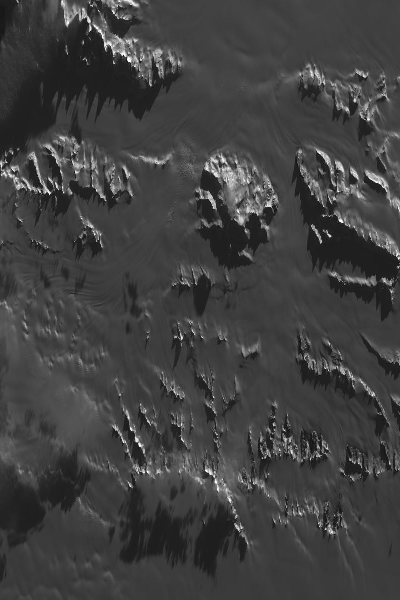
\includegraphics[width=3.0in]{images/examples/spot5_preview.png}
  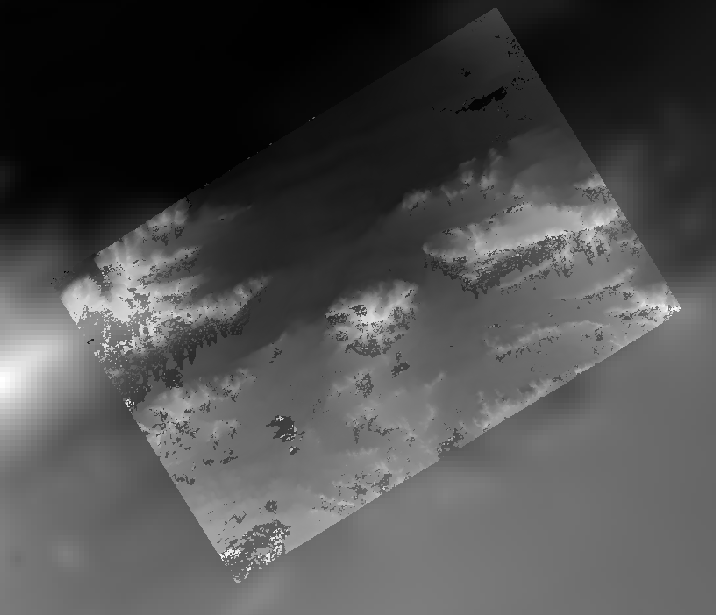
\includegraphics[width=3.0in]{images/examples/spot5_dem.png}
\caption{Cropped region of SPOT5 image and a portion of the associated stereo 
         DEM overlaid on a low resolution Bedmap2 DEM.}
\label{fig:spot5_output}
\end{figure}

\section{Dawn (FC) Framing Camera}

This is a NASA mission to visit two of the largest objects in the
asteroid belt, Vesta and Ceres. The framing camera on board Dawn is
quite small and packs only a resolution of 1024x1024 pixels. This means
processing time is extremely short. To its benefit, it seems that the
mission planners leave the framing camera on taking shots quite
rapidly. On a single pass, they seem to usually take a chain of FC
images that have a high overlap percentage. This opens the idea of using
ASP to process not only the sequential pairs, but also the wider
baseline shots. Then someone could potentially average all the DEMs
together to create a more robust data product.

For this example, we downloaded the images

\begin{center}
\texttt{FC21A0010191\_11286212239F1T.IMG} and
\texttt{FC21A0010192\_11286212639F1T.IMG}
\end{center}

which show the Cornelia crater. We found these images by looking at the
popular anaglyph shown on the Planetary Science Blog
\cite{planetaryblog:vesta}.

\begin{figure}[h!]
\centering
  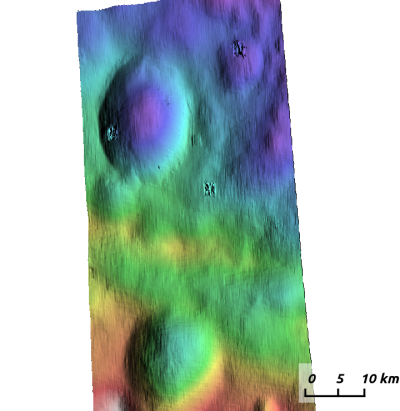
\includegraphics[width=3.0in]{images/examples/dawn/VestaDEMRender_400px.png}
  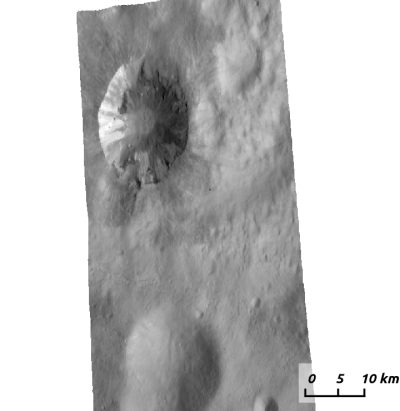
\includegraphics[width=3.0in]{images/examples/dawn/VestaDRGRender_400px.png}
\caption{Example colorized height map and ortho image output.}
\label{fig:dawn-nomap-example}
\end{figure}

\subsubsection*{Commands}

First you must download the Dawn FC images from PDS.

\begin{verbatim}
    ISIS3 > dawnfc2isis from=FC21A0010191_11286212239F1T.IMG \
                        to=FC21A0010191_11286212239F1T.cub
    ISIS3 > dawnfc2isis from=FC21A0010192_11286212639F1T.IMG \
                        to=FC21A0010192_11286212639F1T.cub
    ISIS3 > spiceinit from=FC21A0010191_11286212239F1T.cub
    ISIS3 > spiceinit from=FC21A0010192_11286212639F1T.cub
    ISIS3 > stereo FC21A0010191_11286212239F1T.cub \
                   FC21A0010192_11286212639F1T.cub stereo/stereo
    ISIS3 > point2dem stereo-PC.tif --orthoimage stereo-L.tif \
   --t_srs "+proj=eqc +lat_ts=-11.5 +a=280000 +b=229000 +units=m"
\end{verbatim}

\subsubsection*{stereo.default}

The stereo.default example file (appendix \ref{ch:stereodefault})
works well for this stereo pair. Just set
\texttt{alignment-method} to \texttt{affineepipolar} or
\texttt{homography}.


\section{ASTER Imagery}
\label{sec:aster}

In this example we will describe how to process ASTER Level 1A VNIR imagery. 
The data can be obtained for free from 
\url{https://search.earthdata.nasa.gov/search}. Select a region on the map,
search for AST\_L1A, and choose 
``ASTER L1A Reconstructed Unprocessed Instrument Data V003''.
(The same interface can be used to obtain pre-existing ASTER DEMs.)

There are two important things to keep in mind when ordering the data.
First, at the very last step, when finalizing the order options, 
choose GeoTIFF as the data format, rather than HDF-EOS. 
This way the imagery and metadata will come already extracted from the HDF file.

Second, note that ASP cannot process ASTER Level 1B imagery, as those
images lack camera information.

Below, we will use the dataset
\texttt{AST\_L1A\_00307182000191236\_20160404141337\_21031} near San Luis
Reservoir in Northern California. This dataset will come as a directory
containing TIFF imagery and meta-information as text files. We use the
tool \texttt{aster2asp} (section \ref{app:aster}) to parse it (also
there is described the data contained in this directory):

\begin{verbatim}
  aster2asp 030353697511879 -o out
\end{verbatim}

This command will create 4 files, named

\begin{verbatim}
  out-Band3N.tif out-Band3B.tif out-Band3N.xml out-Band3B.xml
\end{verbatim}

We refer again to the tool's documentation page
regarding details of how these files were created.

Next, we run stereo. We can use either the exact camera model
(\texttt{-t aster}), or its RPC approximation (\texttt{-t rpc}). The
former is much slower but more accurate. 
\begin{verbatim}
  stereo -t aster --subpixel-mode 3 out-Band3N.tif out-Band3B.tif \
     out-Band3N.xml out-Band3B.xml out_stereo/run
\end{verbatim}
or 
\begin{verbatim}
  stereo -t rpc --subpixel-mode 3 out-Band3N.tif out-Band3B.tif \
     out-Band3N.xml out-Band3B.xml out_stereo/run
\end{verbatim}

This is followed by DEM creation:
\begin{verbatim}
  point2dem -r earth --tr 0.000277777777778 out_stereo/run-PC.tif
\end{verbatim}

The value 0.000277777777778 is the desired output DEM resolution, specified in
degrees. It is approximately 31 meters/pixel, the same as the publicly available ASTER DEM,
and about twice the 15 meters/pixel image resolution.

Much higher quality results, but still not as detailed as the public ASTER DEM
can be obtained by doing stereo as before, followed by map-projection onto a coarser and smoother
version of the obtained DEM, and then redoing stereo with map-projected images
(per the suggestions in chapter \ref{tips}).
Using \texttt{-\/-subpixel-mode 2}, while much slower, yields the best results.
The flow is as follows:

\begin{verbatim}
  # Initial stereo
  stereo -t aster --subpixel-mode 3 out-Band3N.tif out-Band3B.tif \
     out-Band3N.xml out-Band3B.xml out_stereo/run               

  # Create a coarse and smooth DEM at 300 meters/pixel
  point2dem -r earth --tr 0.0026949458523585 out_stereo/run-PC.tif \
    -o out_stereo/run-300m

  # Map-project onto this DEM at 10 meters/pixel
  mapproject --tr 0.0000898315284119 out_stereo/run-300m-DEM.tif \
    out-Band3N.tif out-Band3N.xml out-Band3N_proj.tif            
  mapproject --tr 0.0000898315284119 out_stereo/run-300m-DEM.tif \
    out-Band3B.tif out-Band3B.xml out-Band3B_proj.tif            
  
  # Run stereo with the map-projected images with subpixel-mode 2
  stereo -t aster --subpixel-mode 2 out-Band3N_proj.tif out-Band3B_proj.tif \
    out-Band3N.xml out-Band3B.xml out_stereo_proj/run              \
    out_stereo/run-300m-DEM.tif

  # Create the final DEM
  point2dem -r earth --tr 0.000277777777778 out_stereo_proj/run-PC.tif
\end{verbatim}

Here we could have again used \texttt{-t rpc} instead of \texttt{-t aster}.
The map-projection was done using \texttt{-\/-tr 0.0000898315284119}
which is about 10 meters/pixel.

It is possible to increase the resolution of the final DEM slightly
by instead map-projecting at 7 meters/pixel, hence using

\begin{verbatim}
  --tr .0000628820698883
\end{verbatim}

or smaller correlation and subpixel-refinement kernels, that is

\begin{verbatim}
  --corr-kernel 15 15 --subpixel-kernel 25 25
\end{verbatim}

instead of the defaults (21 21 and 35 35) but this comes with increased noise as well, and
using a finer resolution results in longer run-time.

We also tried to first bundle-adjust the cameras, using ASP's \texttt{bundle\_adjust}.
We did not notice a noticeable improvement in results. 

\section{SkySat Imagery}
\label{sec:skysat}

In this section we will discuss how to process the SkySat ``Video'' product. 

It is very important to note that this is a very capricious dataset,
so some patience will be needed to work with it. That is due to the following factors:
\begin{itemize}
 \item The baseline can be small, so the perspective of the left and
  right image can be too similar. 
 \item The footprint on the ground is small, on the order of 2 km.
  \item The terrain can be very steep.
 \item The known longitude-latitude corners of each image have only a few digits of
precision, which can result in poor initial estimatd cameras.
\end{itemize}

Below a recipe for how to deal with this data is described, together with
things to watch for and advice when things don't work. 

\subsection{The input data}

We will use as an illustration a
mountainous terrain close to Breckenridge, Colorado. The dataset we
fetched is called \texttt{s4\_20181107T175036Z\_video.zip}. We chose to
work with the following four images from it:

\begin{verbatim}
  1225648254.44006968_sc00004_c1_PAN.tiff
  1225648269.40892076_sc00004_c1_PAN.tiff
  1225648284.37777185_sc00004_c1_PAN.tiff
  1225648299.37995577_sc00004_c1_PAN.tiff
\end{verbatim}

A sample picture from this image set is
shown in figure \ref{skysat-example}.

It is very important to pick images that have sufficient difference in
perspective, but which are still reasonably similar, as otherwise the
procedure outlined in this section will fail. 

\begin{figure}[h!]
\centering
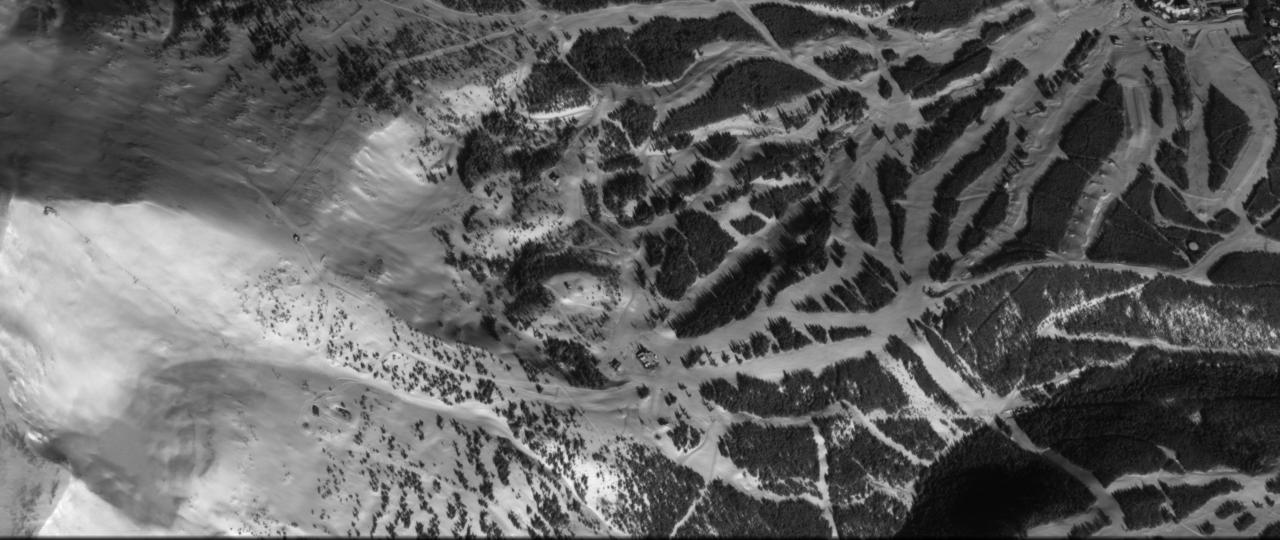
\includegraphics[width=5.0in]{images/Breckenridge.jpg}
\caption{An image used in the SkySat example. Reproduced with permission.}
\label{skysat-example}
\end{figure}

\subsection{Initial camera models and a reference DEM}
\label{refdem}

Based on vendor's documentation, these images are $2560 \times 1080$
pixels.  We use the geometric center of the image as the optical center,
which turned out to be a reasonable enough assumption (verified by
allowing it to float later). Since the focal length is given as 3.6~m and
the pixel pitch is $6.5 \times 10^{-6}$~m, the focal length in pixels is
$$
  3.6/6.5 \times 10^{-6} = 553846.153846. 
$$

We will fetch an SRTM DEM of the area, which will be used as a reference
for registration, from location: 

\begin{verbatim}
  https://e4ftl01.cr.usgs.gov/provisional/MEaSUREs/NASADEM/NorthAmerica/hgt_merge/n39w107.hgt.zip
\end{verbatim}

After unzipping it, we clip it to the area of interest:

\begin{verbatim}
  gdal_translate -projwin -106.1679167 39.5120833 -106.0034722 39.3895833 \
    n39w107.hgt ref_dem_clipped.tif
\end{verbatim}

It is good to be a bit generous with clipping, so that the output DEM
goes a few km or more beyond the region of interest. If the region of
interest is not fully covered by an SRTM tile, a neighboring one can be
downloaded as well.  They can be merged with \texttt{dem\_mosaic} and
then cropped as before.

It appears that SRTM stores heights above the geoid, rather than above the datum.
Hence it needs to be adjusted, as follows:

\begin{verbatim}
  dem_geoid --reverse-adjustment ref_dem_clipped.tif -o -o run/run 
  mv run/run-adj.tif ref_dem.tif
\end{verbatim}

This may adjust the DEM by up to 100 meters. 

Using the tool \texttt{cam\_gen} (section \ref{camgen}) 
bundled with ASP, we create an initial camera model and a GCP file (section \ref{bagcp})
for the first image as as follows:

\begin{verbatim}
  cam_gen output/video/frames/1225648254.44006968_sc00004_c1_PAN.tiff   \
    --reference-dem ref_dem.tif --focal-length 553846.153846            \
    --optical-center 1280 540 --pixel-pitch 1 --height-above-datum 4000 \
    --refine-camera --frame-index output/video/frame_index.csv          \
    --gcp-std 1 -o v1.tsai --gcp-file v1.gcp
\end{verbatim}

This tool works by reading the longitude and latitude of each image corner on the ground 
from the meta file \texttt{frame\_index.csv}, and finding the position and orientation
of the camera that best fits this data. The camera is written to \texttt{v1.tsai}. 
A GCP file is written to \texttt{v1.gcp}. This will help later with bundle adjustment.

In this command, the optical center and focal length are as mentioned
earlier. The reference SRTM DEM is used to infer the height above datum
for each image corner based on its longitude and latitude. The height
value specified via \texttt{-\/-height-above-datum} is used as a
fallback option, if for example, the DEM is incomplete, and is not
strictly necessary for this example. This tool also accepts the
longitude and latitude of the corners as an option, via
\texttt{-\/-lon-lat-values}.

The flag \texttt{-\/-refine-camera} makes \texttt{cam\_gen} solve a least
square problem to refine the output camera. In some rare cases it can get the
refinement wrong, though by and large it it greatly improves the cameras.

For simplicity of notation, we will create a symbolic link from this image to
the shorter name \texttt{v1.tif}, and the GCP file needs to be edited to
reflect this. The same will apply to the other files. We will have then
four images, \texttt{v1.tif, v2.tif, v3.tif, v4.tif}, and corresponding
camera and GCP files.

A good sanity check is to visualize these computed cameras in ASP's
\texttt{orbitviz} tool. It can be invoked as:
\begin{verbatim}
   orbitviz v[1-4].tif v[1-4].tsai -o orbit.kml
\end{verbatim}

The output KML file can then be opened in Google Earth. We very strongly
recommend this step, since it may catch inaccurate cameras which will
cause problems later.

Another important check is to map-project these images using the cameras
and overlay them in \texttt{stereo\_gui} on top of the reference
DEM. Here is an example for the first image:
\begin{verbatim}
  mapproject --t_srs \
  '+proj=stere +lat_0=39.4702 +lon_0=253.908 +k=1 +x_0=0 +y_0=0 +datum=WGS84 +units=m' \
  ref_dem.tif v1.tif v1.tsai v1_map.tif 
\end{verbatim}

Notice that we used above a longitude and latitude around the area of interest. This 
will need to be modified for your specific example. 

\subsection{Bundle adjustment}

At this stage, the cameras should be about right, but not quite
exact. We will take care of this using bundle adjustment. 
We will invoke this tool twice. In the first call we will make the
cameras self-consistent, which can make them move away, however,
and in the second call we will bring them back to the original location.

\begin{verbatim}
  parallel_bundle_adjust -t pinhole --disable-tri-ip-filter \
    --disable-pinhole-gcp-init --skip-rough-homography      \
    --force-reuse-match-files --ip-inlier-factor 1.0        \
    --ip-uniqueness-threshold 0.9 --ip-per-tile 2000        \
    --datum wgs84 --inline-adjustments --camera-weight 0    \
    --overlap-limit 10 --robust-threshold 10                \
    --remove-outliers-params '75 3 5 6'                     \
    --num-passes 2 --num-iterations 1000                    \
    v[1-4].tif v[1-4].tsai -o ba/run

  parallel_bundle_adjust -t pinhole --datum wgs84          \
    --inline-adjustments --num-passes 1                    \
    --num-iterations 0 --transform-cameras-using-gcp       \
    v[1-4].tif ba/run-v[1-4].tsai v[1-4].gcp -o ba/run
\end{verbatim}

The output optimized cameras will be named \texttt{ba/run-run-v[1-4].tsai}.
The reason one has the word ``run'' twice is because we ran 
this tool twice. The intermediate cameras from the first run 
were called \texttt{ba/run-v[1-4].tsai}.

Here we use \texttt{-\/-ip-per-tile 2000} to create a lot of interest
points. This will help with alignment later. It is suggested that the
user study all these options and understand what they do. 
One can also experiment with more than one pass of bundle adjustment,
when outliers are removed. We also used \texttt{-\/-robust-threshold 10}
to force the solver to work the bigger errors. That is necessary
since the initial cameras could be pretty inaccurate. 

It is very important to examine the residual file named
\begin{verbatim}
  ba/run-final_residuals_no_loss_function_pointmap_point_log.csv
\end{verbatim}
Here, the third column are the heights of triangulated interest points,
while the fourth column are the reprojection errors.  Normally these
errors should be a fraction of a pixel, as otherwise the solution did not
converge. The last entries in this file correspond to the GCP, and
those should be looked at carefully as well. The reprojection errors for GCP
should be on the order of tens of pixels because the longitude and latitude
of each GCP are not well-known. 

It is also very important to examine the obtained match files in the 
output directory. If there are too few matches, particularly among very similar
images, one may need to increase the value of \texttt{-\/-ip-inlier-factor}.
Note that a large value here may allow more outliers. 

\subsection{Creating terrain models}
\label{skysat:stereo}

The next step is to run stereo and create DEMs. We will reuse the match files
created and filtered by bundle adjustment as those are likely better
than what stereo can do itself. 

We will run the following command for each pair of images in the bash shell: 
\begin{verbatim}
  i=1
  ((j=i+1))
  st=stereo_v${i}${j}
  rm -rfv $st
  mkdir -p $st
  cp -fv ba/run-v${i}__v${j}-clean.match $st/run-v${i}__v${j}.match
  parallel_stereo --skip-rough-homography -t nadirpinhole --stereo-algorithm 2 \
    v${i}.tif v${j}.tif ba/run-run-v${i}.tsai ba/run-run-v${j}.tsai $st/run
  point2dem --stereographic --proj-lon 253.90793 --proj-lat 39.47021 --tr 4  \
    --errorimage $st/run-PC.tif
\end{verbatim} % Make emacs happy by inserting a $ here.
(Repeat this for other values of $i$.)

Here we chose to use a stereographic projection in \texttt{point2dem}
to create the DEM in units of meter. One can can also use a different
projection that can be passed to the option \texttt{-\/-t\_srs}.

It is important to examine the mean intersection error for each DEM:
\begin{verbatim}
  gdalinfo -stats stereo_v12/run-IntersectionErr.tif |grep Mean
\end{verbatim}

which should hopefully be no more than 0.5 meters, otherwise likely 
bundle adjustment failed. One should also compare the DEMs among themselves:
\begin{verbatim}
  geodiff --absolute stereo_v12/run-DEM.tif stereo_v23/run-DEM.tif -o tmp 
  gdalinfo -stats tmp-diff.tif | grep Mean
\end{verbatim}

Here the mean error should be on the order of 4 meters, or even less. 

\subsection{Mosaicking and alignment}

If more than one image pair was used, the obtained DEMs can be mosaicked:

\begin{verbatim}
  dem_mosaic stereo_v12/run-DEM.tif stereo_v23/run-DEM.tif\
    stereo_v34/run-DEM.tif -o mosaic.tif
\end{verbatim}

This DEM can be hillshaded and overlayed on top of the 
reference DEM.

The next step is aligning it to the reference. 
\begin{verbatim}
  pc_align --max-displacement 1000 --save-transformed-source-points \
    ref_dem.tif mosaic.tif -o align/run
\end{verbatim}

It is important to look at the errors printed by this tool
before and after alignment, as well as details about the alignment
that was applied. The obtained aligned cloud can be made into a DEM again:

\begin{verbatim}
  point2dem --stereographic --proj-lon 253.90793 --proj-lat 39.47021 --tr 4  \
    align/run-trans_source.tif
\end{verbatim}

The absolute difference before and after alignment can be found as 
follows:

\begin{verbatim}
  geodiff --absolute mosaic.tif ref_dem.tif -o tmp 
  gdalinfo -stats tmp-diff.tif | grep Mean
\end{verbatim}

\begin{verbatim}
  geodiff --absolute  align/run-trans_source-DEM.tif ref_dem.tif -o tmp 
  gdalinfo -stats tmp-diff.tif | grep Mean
\end{verbatim}

In this case the mean error after alignemnt was about 7 m, 
which is not too bad given that the reference DEM resolution is about
30 m/pixel.

\subsection{Alignment of cameras}

The transform computed with \texttt{pc\_align} can be used
to bring the cameras in alignment to the reference DEM. That can 
be done as follows:

\begin{verbatim}
  parallel_bundle_adjust -t pinhole --datum wgs84          \
    --inline-adjustments --num-passes 1 --num-iterations 0 \
    --initial-transform align/run-transform.txt            \
    v[1-4].tif ba/run-run-v[1-4].tsai -o ba/run
\end{verbatim}

creating the aligned cameras \texttt{ba/run-run-run-v[1-4].tsai}.

\subsection{Mapprojection}

If the steep topography prevents good DEMs from being created, one can 
map-project the images first onto the reference DEM:

\begin{verbatim}
  for i in 1 2 3 4; do 
    mapproject --t_srs \
     '+proj=stere +lat_0=39.4702 +lon_0=253.908 +k=1 +x_0=0 +y_0=0 +datum=WGS84 +units=m' \
    ref_dem.tif v${i}.tif ba/run-run-run-v${i}.tsai v${i}_map.tif  
  done
\end{verbatim} % put a stray $ here as emacs's highlighting gets confused

and then run stereo with the mapprojected images, such as:

\begin{verbatim}
  i=1
  ((j=i+1))
  stereo v${i}_map.tif v${j}_map.tif                                         \
    ba/run-run-run-v${i}.tsai ba/run-run-run-v${j}.tsai                      \
    stereo_map_v${i}${j}/run ref_dem.tif --session-type pinhole              \
    --cost-mode 4 --stereo-algorithm 2 --corr-seed-mode 1                    \
    --alignment-method none --corr-tile-size 9000                            \
  point2dem --stereographic --proj-lon 253.90793 --proj-lat 39.47021 --tr 4  \
    --errorimage stereo_map_v${i}${j}/run-PC.tif
\end{verbatim}

It is important to note that here we used the cameras that were aligned
with the reference DEM. We could have as well mapprojected onto a
lower-resolution version of the mosaicked and aligned DEM with its holes
filled.

\subsection{When things fail}

Processing SkySat images is difficult, for various reasons mentioned
earlier. A few suggestions were also offered along the way when things
go wrong.

Problems are usually due to cameras being initialized inaccurately
by \texttt{cam\_gen} or bundle adjustment not optimizing them well.
The simplest solution is often to just try a different pair of images from the sequence, 
say from earlier or later in the flight, or a pair with less overlap,
or with more time elapsed between the two acquistions. Modifying various
parameters may help as well.

We have experimented suffiently with various SkySat datasets
to be sure that the intrinsics (focal length, optical center, and pixel pitch)
are usually the issue, rather the positions and orientations of the cameras.

\subsection{Structure from motion}

In case \texttt{cam\_gen} does not create sufficiently good cameras, 
one can attempt to use the \texttt{camera\_solve} tool (chapter \ref{ch:sfm}).
This will create hopefully good cameras but in an arbitrary coordinate system.
Then we will transfer those to the world coordinates using GCP.

Here is an example for two cameras:

\begin{verbatim}
  out=out_v12 
  ba_params="--num-passes 1 --num-iterations 0 --transform-cameras-using-gcp"
\end{verbatim}

\begin{verbatim}
  theia_overdides="--sift_num_levels=6 --lowes_ratio=0.9 
    --min_num_inliers_for_valid_match=10 
    --min_num_absolute_pose_inliers=10 
    --bundle_adjustment_robust_loss_function=CAUCHY 
    --post_rotation_filtering_degrees=180.0 --v=2  
    --max_sampson_error_for_verified_match=100.0 
    --max_reprojection_error_pixels=100.0 
    --triangulation_reprojection_error_pixels=100.0 
    --min_num_inliers_for_valid_match=10 
    --min_num_absolute_pose_inliers=10"                  
\end{verbatim}

\begin{verbatim}
  rm -rfv $out
  camera_solve $out --datum WGS84 --datum WGS84 --calib-file v1.tsai \
      --bundle-adjust-params "$ba_params v1.gcp v2.gcp" v1.tif v2.tif 
\end{verbatim} # make emacs happy $

The obtained cameras would hopefully be good enough to use with stereo,
or they can be used instead of the ones output by \texttt{cam\_gen}
so they can be further bundle-adjusted as at the beginning of the section.

\subsection{RPC models}

Some SkySat datasets come with RPC camera models, typically embedded
in the images. This can be verified by running
\begin{verbatim}
  gdalinfo -stats output/video/frames/1225648254.44006968_sc00004_c1_PAN.tiff
\end{verbatim}

We found that these models are not sufficiently
robust for stereo. But they can be used to create initial guess
cameras with \texttt{cam\_gen} instead of using longitude and latitude
of corners. Here is an example:

\begin{verbatim}
 img=output/video/frames/1225648254.44006968_sc00004_c1_PAN.tiff
 cam_gen $img --reference-dem ref_dem.tif --focal-length 553846.153846  \
    --optical-center 1280 540 --pixel-pitch 1 --height-above-datum 4000 \
    --refine-camera --gcp-std 1 --input-camera $img                     \
    -o v1_rpc.tsai --gcp-file v1_rpc.gcp
\end{verbatim}

and then one can proceed as earlier (particularly the GCP file can be edited
to reflect the shorter image name).

One can also regenerate the provided SkySat RPC model as:

\begin{verbatim}
  cam2rpc -t rpc --dem-file dem.tif input.tif output.xml
\end{verbatim}

Here, the reference DEM should go beyond the extent of the image.  This tool
makes it possible to decide how finely to sample the DEM, and one can
simply use longitude-latitude and height ranges instead of the DEM.

We assumed in the last command that the input image implicitly stores
the RPC camera model, as is the case for SkySat.

Also, any pinhole camera models obtained using our software 
can be converted to RPC models as follows:

\begin{verbatim}
  cam2rpc --dem-file dem.tif input.tif input.tsai output.xml 
\end{verbatim}

\subsection{Bundle adjustment using reference terrain}

At this stage, if desired, but this is rather unnecessary, 
one can do joint optimization of the cameras using dense
and uniformly distributed interest points, and using the reference DEM as a constraint.
This should make the DEMs more consistent among themselves and closer to the reference DEM.

It is also possible to float the intrinsics, per section \ref{floatingintrinsics},
which sometimes can improve the results further. 

For that, one should repeat the \texttt{stereo\_tri} part of
of the stereo commands from section \ref{skysat:stereo}
with the flags 
\texttt{-\/-num-matches-from-disp-triplets 10000} and \
\texttt{-\/-unalign-disparity} to obtain dense interest points
and unaligned disparity. 

The match points can be examined as:
\begin{verbatim}
  stereo_gui v1.tif v2.tif stereo_v12/run-disp-v1__v2.match
\end{verbatim}
and the same for the other image pairs. Hopefully they will fill as much
of the images as possible. One should also study the unaligned disparities,
for example
\begin{verbatim}
  stereo_v12/run-v1__v2-unaligned-D.tif
\end{verbatim}
by invoking \texttt{disparitydebug} on it and then visualizing the two
obtained images. Hopefully these disparities are dense and with few holes. 

The dense interest points should be copied to the new bundle adjustment directory, such as
\begin{verbatim}
  mkdir -p run_ref_terrain
  cp stereo_v12/run-disp-v1__v2.match run_ref_terrain/run-v1__v2.match
\end{verbatim}

and the same for the other ones (note the convention for match files in the new directory).
The unaligned disparities can be used from where they are. 

Then bundle adjustment using the reference terrain constraint proceeds as follows:
\begin{verbatim}
  disp_list=$(ls stereo_v*/*-unaligned-D.tif)
  bundle_adjust v[1-4].tif  ba_align/run-run-v[1-4].tsai -o ba_ref_terrain/run  \
  --reference-terrain ref_dem.tif --disparity-list "$disp_list"                 \
  --max-num-reference-points 10000000 --reference-terrain-weight 50             \ 
  --parameter-tolerance 1e-12 -t nadirpinhole --max-iterations 500              \
  --overlap-limit 1 --inline-adjustments --robust-threshold 2                   \
  --force-reuse-match-files --max-disp-error 100 --camera-weight 0
\end{verbatim}

If invoking this creates new match files, it means that the dense match files 
were not copied successfully to the new location. If this optimization is slow,
perhaps too many reference terrain points were picked. 

This will create, as before, the residual file named
\begin{verbatim}
  ba_ref_terrain/run-final_residuals_no_loss_function_pointmap_point_log.csv
\end{verbatim}
showing how consistent are the cameras among themselves, 
and in addition, a file named
\begin{verbatim}
  ba_ref_terrain/run-final_residuals_no_loss_function_reference_terrain.txt
\end{verbatim}

which tells how well the cameras are aligned to the reference
terrain. The errors in the first file should be under 1 pixel, and in
the second one should be mostly under 2-3 pixels (both are the fourth
column in these files).

The value of \texttt{-\/-reference-terrain-weight} can be increased to make the 
alignment to the reference terrain a little tighter.

It is hoped that after running stereo with these refined cameras, the obtained DEMs
will differ by less than 2~m among themselves, and by less than 4~m as compared
to the reference DEM. 

\subsection{Floating the camera intrinsics}

If desired to float the focal length as part of the optimization, one should 
pass in addition, the options
\begin{verbatim}
 --solve-intrinsics --intrinsics-to-float 'focal_length'
\end{verbatim}
Floating the optical center can be done by adding it in as well. 

It is important to note that for SkySat the intrinsics seem to be already quite good,
and floating them is not necessary and is only shown for completeness. If 
one wants to float them, one should vary the focal length while keeping the optical center
fixed, and vice versa, and compare the results. Then, with the result that shows most
promise, one should vary the other parameter. If optimizing the intrinsics too aggressively,
it is not clear if they will still deliver better results with other images or 
if comparing with a different reference terrain. 

Yet, if desired, one can float even the distortion parameters. 
For that, the input camera files need to be converted
to some camera model having these (see section \ref{pinholemodels}), 
and their values can be set to something very small.
One can use the Brown-Conrady model, for example, so each camera file must have
instead of \texttt{NULL} at the end the fields:
\begin{verbatim}
BrownConrady
xp  = -1e-12
yp  = -1e-12
k1  = -1e-10
k2  = -1e-14
k3  = -1e-22
p1  = -1e-12
p2  = -1e-12
phi = -1e-12
\end{verbatim}

There is always a chance when solving these parameters that the obtained
solution is not optimal.  Hence, one can also try using as initial
guesses different values, for example, by negating the above numbers.

One can also try to experiment with the option
\texttt{-\/-heights-from-dem}, and also with
\texttt{-\/-robust-threshold} if it appears that the large errors are
not minimized enough.

\section{Declassified satellite images: KH-4B}
\label{kh4}

ASP supports the declassified high-resolution CORONA KH-4B images.
These images can be processed using either optical bar (panoramic)
camera models or as pinhole camera models with RPC distortion.
Most of the steps are similar to the example in section \ref{skysat-example}.
The optical bar camera model is based on \cite{schenk2003rigorous} and
\cite{sohn2004mathematical}, whose format is described in section
\ref{panoramic}.

\subsection{Fetching the data}

KH-4B images are available via the USGS Earth Explorer, at
\begin{center}
 \url{https://earthexplorer.usgs.gov/}
\end{center}

(an account is required to download the data). We will work with the KH-4B image pair

\begin{verbatim}
 DS1105-2248DF076
 DS1105-2248DA082
\end{verbatim}

To get these from Earth Explorer, click on the \texttt{Data Sets}
tab and select the three types of declassified data available, then in the 
\texttt{Additional Criteria} tab choose \texttt{Declass 1}, and in
the \texttt{Entity ID} field in that tab paste the above frames (if no results
are returned, one can attempt switching above to \texttt{Declass 2},
etc). Clicking on the \texttt{Results} tab presents the user with information about
these frames.

Clicking on \texttt{Show Metadata and Browse} for every
image will pop-up a table with meta-information. That one can be pasted
into a text file, named for example, \texttt{DS1105-2248DF076.txt} for the
first image, from which later the longitude and latitude of each image corner
will be parsed. Then one can click on \texttt{Download Options} 
to download the data. 

\subsection{Stitching the images}

Each downloaded image will be made up of 2-4 portions, presumably due
to the limitations of the scanning equipment. They can be stitched together
using ASP's \texttt{image\_mosaic} tool (section \ref{imagemosaic}).

For some reason, the KH-4B images are scanned in an unusual order. To
mosaic them, the last image must be placed first, the next to last
should be second, etc. In addition, as seen from the tables of metadata discussed
earlier, some images correspond to the \texttt{Aft} camera type. Those
should be rotated 180 degrees after mosaicking, hence below we use
the \texttt{-\/-rotate} flag for that one.  The overlap width is manually 
determined by looking at two of the sub images in \texttt{stereo\_gui}.

With this in mind, image mosaicking for these two images will happen as follows:

\begin{verbatim}
  image_mosaic DS1105-2248DF076_d.tif  DS1105-2248DF076_c.tif              \
    DS1105-2248DF076_b.tif  DS1105-2248DF076_a.tif -o DS1105-2248DF076.tif \
    --ot byte --overlap-width 7000 --blend-radius 2000
  image_mosaic DS1105-2248DA082_d.tif DS1105-2248DA082_c.tif               \
    DS1105-2248DA082_b.tif  DS1105-2248DA082_a.tif -o DS1105-2248DA082.tif \
    --ot byte --overlap-width 7000 --blend-radius 2000 --rotate
\end{verbatim}

In order to process with the optical bar camera model these images need to be cropped
to remove the most of empty area around the image.  The four corners of the valid image 
area can be manually found by clicking on the corners in \texttt{stereo\_gui}.  Note that
for some input images it can be unclear where the proper location for the corner is due to
edge artifacts in the film.  Do your best to select the image corners such that obvious
artifacts are kept out and all reasonable image sections are kept in.
ASP provides a simple Python tool called \texttt{historical\_helper.py} to rotate the image so that the top edge is horizontal
while also cropping the boundaries.  Pass in the corner coordinates as shown below
in the order top-left, top-right, bot-right, bot-left (column then row).
This is also a good opportunity to simplify the file names going forwards.

\begin{verbatim}
  historical_helper.py rotate-crop --input-path DS1105-2248DA082.tif  --output-path aft.tif \
    --interest-points '4523 1506  114956 1450  114956 9355  4453 9408'
  historical_helper.py rotate-crop --input-path DS1105-2248DF076.tif  --output-path for.tif \
    --interest-points '6335 1093  115555 1315  115536 9205  6265 8992'
\end{verbatim}

\subsection{Fetching a ground truth DEM}

To create initial cameras to use with these images, and to later refine and validate
the terrain model made from them, we will need a ground truth source. 
Several good sets of DEMs exist, including SRTM, ASTER, and TanDEM-X. Here we will
work with SRTM, which provides DEMs with a 30-meter post spacing. The bounds of the region 
of interest are inferred from the tables with meta-information from above. 
We will use \texttt{wget} to fetch
\begin{center}
\url{https://e4ftl01.cr.usgs.gov/provisional/MEaSUREs/NASADEM/Eurasia/hgt_merge/n31e099.hgt.zip}
\end{center}
and also tiles \texttt{n31e100} and \texttt{n31e101}. After unzipping, these can be
merged and cropped as follows:

\begin{verbatim}
  dem_mosaic n*.hgt --t_projwin 99.6 31.5 102 31 -o dem.tif
\end{verbatim}

Determining these bounds and the visualization of all images and DEMs
can be done in \texttt{stereo\_gui}.

The SRTM DEM may need adjustment, as discussed in section \ref{refdem}.

\subsection{Creating camera files}

ASP provides the tool named \texttt{cam\_gen} that, based on a camera's intrinsics
and the positions of the image corners on Earth's surface will
create initial camera models that will be the starting point for aligning the cameras.

To create optical bar camera models, an example camera model file is needed.
This needs to contain all of the expected values for the camera, though
image\_size, image\_center, iC, and IR can be any value since they will be recalculated.
The pitch is determined by the resolution of the scanner used, which is seven microns.
The other values are determined by looking at available information about the satellite.
For the first image (DS1105-2248DF076) the following values were used:

\begin{verbatim}
  VERSION_4
  OPTICAL_BAR
  image_size = 13656 1033
  image_center = 6828 517
  pitch = 7.0e-06
  f = 0.61000001430511475
  scan_time = 0.5
  forward_tilt = 0.2618
  iC = -1030862.1946224371 5468503.8842079658 3407902.5154047827
  iR = -0.95700845635275322 -0.27527006183758934 0.091439638698163225 \
       -0.26345593052063937 0.69302501329766897 -0.67104940475144637 \
       0.1213498543172795 -0.66629027007731101 -0.73575232847574434
  speed = 7700
  mean_earth_radius = 6371000
  mean_surface_elevation = 4000
  motion_compensation_factor = 1.0
  scan_dir = right
\end{verbatim}

For a description of each value, see \ref{panoramic}.
For the other image (aft camera) the forward tilt was set to -0.2618 and scan\_dir was set to 'left'.
The correct values for scan\_dir (left or right) and use\_motion\_compensation (1.0 or -1.0) are not
known for certain due to uncertainties about how the images were recorded and may even change
between launches of the KH-4 satellite.  You will need to experiment to see which combination of settings
produces the best results for your particular data set.

The metadata table from Earth Explorer has the following entries
for DS1105-2248DF076:
\begin{verbatim}
  NW Corner Lat dec   31.266
  NW Corner Long dec  99.55
  NE Corner Lat dec   31.55
  NE Corner Long dec  101.866
  SE Corner Lat dec   31.416
  SE Corner Long dec  101.916
  SW Corner Lat dec   31.133
  SW Corner Long dec  99.55
\end{verbatim}

These correspond to the upper-left, upper-right, lower-right, and lower-left
pixels in the image. We will invoke \texttt{cam\_gen} as follows:

\begin{verbatim}
  cam_gen --sample-file sample_kh4b_for_optical_bar.tsai --camera-type opticalbar \
    --lon-lat-values '99.55 31.266 101.866 31.55 101.916 31.416 99.55 31.133' \
    for.tif --reference-dem dem.tif --refine-camera -o for.tsai

  cam_gen --sample-file sample_kh4b_aft_optical_bar.tsai --camera-type opticalbar
    --lon-lat-values '99.566 31.266 101.95 31.55 101.933 31.416 99.616 31.15' \
    aft.tif --reference-dem dem.tif --refine-camera -o aft.tsai
\end{verbatim}

It is very important to note that if, for example, the upper-left image
corner is in fact the NE corner from the metadata, then that corner 
should be the first in the longitude-latitude list when invoking this tool.

An important sanity check is to mapproject the images with these
cameras, for example as:

\begin{verbatim}
  mapproject dem.tif for.tif for.tsai for.map.tif
\end{verbatim}

and then overlay the mapprojected image on top of the DEM in \texttt{stereo\_gui}.
If it appears that the image was not projected correctly, likely 
the order of image corners was incorrect. At this stage it is not unusual
that the mapprojected images are shifted from where they should be, that
will be corrected later. 

\subsection{Bundle adjustment and stereo}

Before processing the input images it is a good idea to experiment with
reduced resolution copies in order to accelerate testing.  You can easily
generate reduced resolution copies of the images using \texttt{stereo\_gui}
as shown below.  When making a copy of the camera model files, make sure to
update image\_size, image\_center (divide by N), and the pitch (multiply by N)
to account for the downsample amount.

\begin{verbatim}
  stereo_gui for.tif aft.tif --create-image-pyramids-only
  ln -s for_sub8.tif  for_small.tif
  ln -s aft_sub8.tif  aft_small.tif
  cp for.tsai  for_small.tsai
  cp aft.tsai  aft_small.tsai
\end{verbatim}

You can now run bundle adjustment on the downsampled images:

\begin{verbatim}
  bundle_adjust for_small.tif aft_small.tif                 \
    for_small.tsai aft_small.tsai                           \
    -o ba_small/run --max-iterations 100 --camera-weight 0  \
    --disable-tri-ip-filter --disable-pinhole-gcp-init      \
    --skip-rough-homography --inline-adjustments            \
    --ip-detect-method 1 -t opticalbar --datum WGS84
\end{verbatim}

Followed by stereo and DEM creation:

\begin{verbatim}
  parallel_stereo for_small.tif aft_small.tif                        \
    ba_small/run-for_small.tsai ba_small/run-aft_small.tsai          \
    stereo_small_mgm/run --alignment-method affineepipolar           \
    -t opticalbar --skip-rough-homography --disable-tri-ip-filter  \
    --skip-low-res-disparity-comp --ip-detect-method 1               \
    --stereo-algorithm 2 

  point2dem --stereographic --proj-lon 100.50792 --proj-lat 31.520417 \
    --tr 30 stereo_small_mgm/run-PC.tif
\end{verbatim}

This will create a very rough initial DEM. It is sufficient however
to align and compare with the SRTM DEM:

\begin{verbatim}
  pc_align --max-displacement -1                                      \
    --initial-transform-from-hillshading similarity                   \
    --save-transformed-source-points --num-iterations 0               \
    --max-num-source-points 1000 --max-num-reference-points 1000      \
    dem.tif stereo_small_mgm/run-DEM.tif -o stereo_small_mgm/run

  point2dem --stereographic --proj-lon 100.50792 --proj-lat 31.520417 \
    --tr 30 stereo_small_mgm/run-trans_source.tif
\end{verbatim}

This will hopefully create a DEM aligned to the underlying SRTM. There
is a chance that this may fail as the two DEMs to align could be too
different. In that case, one can re-run \texttt{point2dem} to re-create
the DEM to align with a coarser resolution, say with \texttt{-\/-tr
120}, then re-grid the SRTM DEM to the same resolution, which can be
done as:

\begin{verbatim}
  pc_align --max-displacement -1 dem.tif dem.tif -o dem/dem             \
    --num-iterations 0 --max-num-source-points 1000                     \
    --max-num-reference-points 1000 --save-transformed-source-points

  point2dem --stereographic --proj-lon 100.50792 --proj-lat 31.520417   \
    --tr 120 dem/dem-trans_source.tif
\end{verbatim}

You can then try to align the newly obtained coarser SRTM DEM to the 
coarser DEM from stereo. 

\subsection{Floating the intrinsics}

The obtained alignment transform can be used to align 
the cameras as well, and then one can experiment with 
floating the intrinsics, as in section \ref{sec:skysat}.

\subsection{Modeling the camera models as pinhole cameras with RPC distortion}

Once sufficiently good optical bar cameras are produced and the DEMs
from them are reasonably similar to some reference terrain ground truth,
such as SRTM, one may attempt to improve the accuracy further by
modeling these cameras as simple pinhole models with the nonlinear
effects represented as a distortion model given by Rational Polynomial
Coefficients (RPC) of any desired degree (see section
\ref{pinholemodels}). The best fit RPC representation can be found for
both optical bar models, and the RPC can be further optimized using the
reference DEM as a constraint.

To convert from optical bar models to pinhole models with RPC distortion
one does

\begin{verbatim}
   convert_pinhole_model for_small.tif for_small.tsai -o for_small_rpc.tsai \
     --output-type RPC --sample-spacing 50 --rpc-degree 2
\end{verbatim}

and the same for the other camera. The obtained cameras should be
bundle-adjusted as before. One can create a DEM and compare
it with the one obtained with the earlier cameras. Likely 
some shift in the position of the DEM will be present, but hopefully 
not too large. The \texttt{pc\_align} tool can be used 
to make this DEM aligned to the reference DEM. 

Next, one follows the same process as outlined in sections
\ref{sec:skysat} and \ref{floatingintrinsics} to refine the RPC
coefficients. We will float the RPC coefficients of the left and
right images independently, as they are unrelated. Hence the command
we will use is:

\begin{verbatim}
  bundle_adjust for_small.tif aft_small.tif for_small_rpc.tsai aft_small_rpc.tsai \
    -o ba_rpc/run --max-iterations 200 --camera-weight 0                          \
    --disable-tri-ip-filter --disable-pinhole-gcp-init                            \
    --skip-rough-homography --inline-adjustments                                  \
    --ip-detect-method 1 -t nadirpinhole --datum WGS84                            \
    --force-reuse-match-files --reference-terrain-weight 1000                     \
    --parameter-tolerance 1e-12 --max-disp-error 100                              \
    --disparity-list stereo/run-unaligned-D.tif                                   \
    --max-num-reference-points 40000 --reference-terrain srtm.tif                 \
    --solve-intrinsics --intrinsics-to-share 'focal_length optical_center'        \
    --intrinsics-to-float other_intrinsics --robust-threshold 10                  \
    --initial-transform pc_align/run-transform.txt
\end{verbatim}

Here it is suggested to use a match file with dense interest points.
The initial transform is the transform written by \texttt{pc\_align}
applied to the reference terrain and the DEM obtained with the camera
models \texttt{for\_small\_rpc.tsai} and \texttt{aft\_small\_rpc.tsai}
(with the reference terrain being the first of the two clouds passed to
the alignment program). The unaligned disparity in the disparity list
should be from the stereo run with these initial guess camera models
(hence stereo should be used with the \texttt{--\/-unalign-disparity}
option). It is suggested that the optical center and focal lengths of
the two cameras be kept fixed, as RPC distortion should be able model
any changes in those quantities as well.

One can also experiment with the option \texttt{-\/-heights-from-dem}
instead of \texttt{-\/-reference-terrain}. The former seems to be able
to handle better large height differences between the 
DEM with the initial cameras and the reference terrain, while the 
former is better at refining the solution. 

Then one can create a new DEM from the optimized camera models and see
if it is an improvement.

\section{Declassified satellite images: KH-7}
\label{kh7}

KH-7 was an effective observation satellite that followed the Corona program.
It contained an index (frame) camera and a single strip (pushbroom) camera.
ASP does currently have a dedicated camera model for this camera, so we will
have to try to approximate it with a pinhole model.  Without a dedicated solution
for this camera, you may only be able to get good results near the central region
of the image.

For this example we find the following images in Earth Explorer declassified collection 2:
\begin{verbatim}
  DZB00401800038H025001
  DZB00401800038H026001
\end{verbatim}

Make note of the lat/lon corners of the images listed in Earth Explorer, and note which
image corners correspond to which compass locations.

After downloading and unpacking the images, we merge them with the \texttt{image\_mosaic} tool.
These images have a large amount of overlap and we need to manually lower the blend radius so
that we do not have memory problems when merging the images.  Note that the image order is 
different for each image.

\begin{verbatim}
  image_mosaic DZB00401800038H025001_b.tif  DZB00401800038H025001_a.tif      \
    -o DZB00401800038H025001.tif  --ot byte --blend-radius 2000  --overlap-width 10000 \
  image_mosaic DZB00401800038H026001_a.tif  DZB00401800038H026001_b.tif      \
    -o DZB00401800038H026001.tif  --ot byte --blend-radius 2000  --overlap-width 10000 \
\end{verbatim}

For this image pair we will use the following SRTM images from Earth Explorer:

\begin{verbatim}
  n22_e113_1arc_v3.tif
  n23_e113_1arc_v3.tif
  dem_mosaic n22_e113_1arc_v3.tif n23_e113_1arc_v3.tif -o srtm_dem.tif
\end{verbatim}

(The SRTM DEM may need adjustment, as discussed in section \ref{refdem}.)

Next we crop the input images so they only contain valid image area.

\begin{verbatim}
  historical_helper.py rotate-crop --input-path DZB00401800038H025001.tif \
  --output-path 5001.tif  --interest-points '1847 2656  61348 2599  61338 33523  1880 33567'
  historical_helper.py rotate-crop --input-path DZB00401800038H026001.tif \
  --output-path 6001.tif  --interest-points '566 2678  62421 2683  62290 33596  465 33595'
\end{verbatim}


We will try to approximate the KH7 camera using a pinhole model.
The pitch of the image is determined by the scanner, which is 7.0e-06 meters per pixel.
The focal length of the camera is reported to be 1.96 meters, and we will set the optical
center at the center of the image.  We need to convert the optical center to units of meters,
which means multiplying the pixel coordinates by the pitch to get units of meters.

Using the image corner coordinates which we recorded earlier, use the \texttt{cam\_gen}
tool to generate camera models for each image, being careful of the order of coordinates.

\begin{verbatim}
  cam_gen --pixel-pitch 7.0e-06 --focal-length 1.96                                 \
    --optical-center 0.2082535  0.1082305                                           \
    --lon-lat-values '113.25 22.882  113.315 23.315  113.6 23.282  113.532 22.85'   \
    5001.tif --reference-dem srtm_dem.tif --refine-camera -o 5001.tsai
  cam_gen --pixel-pitch 7.0e-06 --focal-length 1.96                                 \
    --optical-center 0.216853 0.108227                                              \
    --lon-lat-values '113.2 22.95  113.265 23.382  113.565 23.35  113.482 22.915'   \
    6001.tif --reference-dem srtm_dem.tif --refine-camera  -o 6001.tsai
\end{verbatim}


A quick way to evaluate the camera models is to use the \texttt{camera\_footprint} tool to
create KML footprint files, then look at them in Google Earth.  For a more detailed view,
you can map project them and overlay them on the reference DEM in \texttt{stereo\_gui}.

\begin{verbatim}
  camera_footprint 5001.tif  5001.tsai  --datum  WGS_1984 --quick \
    --output-kml  5001_footprint.kml -t nadirpinhole --dem-file srtm_dem.tif
  camera_footprint 6001.tif  6001.tsai  --datum  WGS_1984 --quick \
    --output-kml  6001_footprint.kml -t nadirpinhole --dem-file srtm_dem.tif
\end{verbatim}

The output files from \texttt{cam\_gen} will be roughly accurate but they may still be bad
enough that \texttt{bundle\_adjust} has trouble finding a solution.  One way to improve your
initial models is to use ground control points.  For this test case I was able to match
features along the rivers to the same rivers in a hillshaded version of the reference DEM.
I used three sets of GCPs, one for each image individually and a joint set for both images.
I then ran \texttt{bundle\_adjust} individually for each camera using the GCPs.

\begin{verbatim}
  bundle_adjust 5001.tif 5001.tsai gcp_5001.gcp -t nadirpinhole --inline-adjustments \
    --num-passes 1 --camera-weight 0 --ip-detect-method 1 -o bundle_5001/out       \
    --max-iterations 30 --fix-gcp-xyz

  bundle_adjust 6001.tif 6001.tsai gcp_6001.gcp -t nadirpinhole --inline-adjustments \
    --num-passes 1 --camera-weight 0 --ip-detect-method 1 -o bundle_6001/out       \
    --max-iterations 30 --fix-gcp-xyz
\end{verbatim}

At this point it is a good idea to experiment with downsampled copies of the input
images before running processing with the full size images.  You can generate these 
using \texttt{stereo\_gui}.  Also make copies of the camera model
files and scale the image center and pitch to match the downsample amount.

\begin{verbatim}
  stereo_gui 5001.tif 6001.tif --create-image-pyramids-only
  ln -s 5001_sub16.tif  5001_small.tif
  ln -s 6001_sub16.tif  6001_small.tif
  cp 5001.tsai  5001_small.tsai
  cp 6001.tsai  6001_small.tsai
\end{verbatim}

Now we can run \texttt{bundle\_adjust} and \texttt{stereo}.  If you are using the
GCPs from earlier, the pixel values will need to be scaled to match the downsampling
applied to the input images.

\begin{verbatim}
  bundle_adjust 5001_small.tif 6001_small.tif bundle_5001/out-5001_small.tsai \
    bundle_6001/out-6001_small.tsai gcp_small.gcp -t nadirpinhole               \
    -o bundle_small_new/out --force-reuse-match-files --max-iterations 30     \
    --camera-weight 0 --disable-tri-ip-filter --disable-pinhole-gcp-init      \
    --skip-rough-homography --inline-adjustments --ip-detect-method 1         \
    --datum WGS84 --num-passes 2

  stereo --alignment-method homography --skip-rough-homography              \
    --disable-tri-ip-filter --ip-detect-method 1 --session-type nadirpinhole  \
     5001_small.tif 6001_small.tif bundle_small_new/out-out-5001_small.tsai \
    bundle_small_new/out-out-6001_small.tsai st_small_new/out

  gdal_translate -b 4 st_small_new/out-PC.tif st_small_new/error.tif
\end{verbatim}


Looking at the error result, it is clear that the simple pinhole model is not
doing a good job modeling the KH7 camera.  We can try to improve things by
adding a distortion model to replace the NULL model in the .tsai files we are using.

\begin{verbatim}
BrownConrady
xp  = -1e-12
yp  = -1e-12
k1  = -1e-10
k2  = -1e-14
k3  = -1e-22
p1  = -1e-12
p2  = -1e-12
phi = -1e-12
\end{verbatim}

Once the distortion model is added, you can use \texttt{bundle\_adjust} to optimize
them.  See the section on solving for pinhole intrinsics in the KH4B example for details.
We hope to provide a more rigorous method of modeling the KH7 camera in the future.


\section{Declassified satellite images: KH-9}
\label{kh9}

The KH-9 satellite contained one frame camera and two panoramic cameras,
one pitched forwards and one aft.  The frame camera is a normal pinhole model so
this example describes how to set up the panoramic cameras for processing.
Processing this data is similar to processing KH-4B data except that the 
images are much larger.

For this example we use the following images from the Earth Explorer declassified collection 3:
\begin{verbatim}
  D3C1216-200548A041
  D3C1216-200548F040
\end{verbatim}

Make note of the lat/lon corners of the images listed in Earth Explorer, and note which
image corners correspond to which compass locations.

After downloading and unpacking the images, we merge them with the \texttt{image\_mosaic} tool.

\begin{verbatim}
  image_mosaic D3C1216-200548F040_a.tif  D3C1216-200548F040_b.tif  D3C1216-200548F040_c.tif \
    D3C1216-200548F040_d.tif  D3C1216-200548F040_e.tif  D3C1216-200548F040_f.tif            \
    D3C1216-200548F040_g.tif  D3C1216-200548F040_h.tif  D3C1216-200548F040_i.tif            \
    D3C1216-200548F040_j.tif  D3C1216-200548F040_k.tif  D3C1216-200548F040_l.tif            \
    --ot byte --overlap-width 3000 -o D3C1216-200548F040.tif
  image_mosaic D3C1216-200548A041_a.tif  D3C1216-200548A041_b.tif  D3C1216-200548A041_c.tif \
    D3C1216-200548A041_d.tif  D3C1216-200548A041_e.tif  D3C1216-200548A041_f.tif            \
    D3C1216-200548A041_g.tif  D3C1216-200548A041_h.tif  D3C1216-200548A041_i.tif            \
    D3C1216-200548A041_j.tif  D3C1216-200548A041_k.tif --overlap-width 1000                 \
    --ot byte -o D3C1216-200548A041.tif  --rotate
\end{verbatim}

These images also need to be cropped to remove most of the area around the images:

\begin{verbatim}
  historical_helper.py rotate-crop --input-path D3C1216-200548F040.tif --output-path for.tif \
    --interest-points '2414 1190  346001 1714  345952 23960  2356 23174'
  historical_helper.py rotate-crop --input-path D3C1216-200548A041.tif --output-path aft.tif \
    --interest-points '1624 1333  346183 1812  346212 24085  1538 23504'
\end{verbatim}

For this example there are ASTER DEMs which can be used for reference.  They can be downloaded from
\url{https://gdex.cr.usgs.gov/gdex/} as single GeoTIFF files.  To cover the entire area of this
image pair you may need to download two files separately and merge them using \texttt{dem\_mosaic}.

As with KH-4B, this satellite contains a forward pointing and aft pointing camera that need to have
different values for "forward\_tilt" in the sample camera files.  The suggested values are -0.174533
for the aft camera and 0.174533 for the forward camera.  Note that some KH9 images have a much smaller
field of view (horizontal size) than others!

\begin{verbatim}
  VERSION_4
  OPTICAL_BAR
  image_size = 62546 36633
  image_center = 31273 18315.5
  pitch = 7.0e-06
  f = 1.5
  scan_time = 0.7
  forward_tilt = 0.174533
  iC = -1053926.8825477704 5528294.6575468015 3343882.1925249361
  iR = -0.96592328992496967 -0.16255393156297787 0.20141603042941184 \
       -0.23867502833024612 0.25834753840712932 -0.93610404349651921 \
       0.10013205696518604 -0.95227767417513032 -0.28834146846321851
  speed = 8000
  mean_earth_radius = 6371000
  mean_surface_elevation = 0
  motion_compensation_factor = 1
  scan_dir = right
\end{verbatim}

Camera files are generated using \texttt{cam\_gen} from a sample camera file as in the previous examples.

\begin{verbatim}
  cam_gen --sample-file sample_kh9_for_optical_bar.tsai --camera-type opticalbar          \
    --lon-lat-values '-151.954 61.999  -145.237 61.186  -145.298 60.944  -152.149 61.771' \
    for.tif --reference-dem aster_dem.tif --refine-camera  -o for.tsai
  cam_gen --sample-file sample_kh9_aft_optical_bar.tsai --camera-type opticalbar         \
    --lon-lat-values '-152.124 61.913  -145.211 61.156  -145.43 60.938  -152.117 61.667' \
    aft.tif --reference-dem aster_dem.tif --refine-camera  -o aft.tsai
\end{verbatim}

As with KH-4B, it is best to first experiment with low resolution copies of the images.
Don't forget to scale the image size, center location, and pixel size in the new camera files!

\begin{verbatim}
  stereo_gui for.tif aft.tif --create-image-pyramids-only
  ln -s for_sub32.tif  for_small.tif
  ln -s aft_sub32.tif  aft_small.tif
  cp for.tsai  for_small.tsai
  cp aft.tsai  aft_small.tsai
\end{verbatim}

From this point KH-9 data can be processed in a very similar manner to the KH-4B example.
Once again, you may need to vary some of the camera parameters to find the settings that
produce the best results.  For this example we will demonstrate how to use 
\texttt{bundle\_adjust} to solve for intrinsic parameters in optical bar models.

Using the DEM and the input images it is possible to collect rough ground control points
which can be used to roughly align the initial camera models.

\begin{verbatim}
  bundle_adjust for_small.tif for_small.tsai ground_control_points.gcp -t opticalbar \
    --inline-adjustments --num-passes 1 --camera-weight 0 --ip-detect-method 1       \
    -o bundle_for_small/out --max-iterations 30 --fix-gcp-xyz

  bundle_adjust aft_small.tif aft_small.tsai ground_control_points.gcp -t opticalbar \
    --inline-adjustments --num-passes 1 --camera-weight 0 --ip-detect-method 1       \
    -o bundle_aft_small/out --max-iterations 30 --fix-gcp-xyz
\end{verbatim}

Now we can do a joint bundle adjustment.  While in this example we immediately attempt
to solve for intrinsics, you can get better results using techniques such as the
\texttt{-\/-disparity-list} option described in \ref{kh4} and \ref{sec:skysat} along with
the reference DEM.  We will try to solve for all intrinsics but will share the
focal length and optical center since we expect them to be very similar.  If we get
good values for the other intrinsics we could do another pass where we don't share
those values in order to find small difference between the two cameras.  We specify
intrinsic scaling limits here.  The first three pairs are for the focal length and
the two optical center values.  For an optical bar camera, the next three values are
for \texttt{speed}, \texttt{motion\_compensation\_factor}, and \texttt{scan\_time}.
We are fairly confident in the focal length and the optical center but we only have
guesses for the other values so we allow them to vary in a wider range.

\begin{verbatim}
  bundle_adjust left_small.tif right_small.tif bundle_for_small/out-for_small.tsai \
    bundle_aft_small/out-aft_small.tsai -t opticalbar -o bundle_small/out          \
    --force-reuse-match-files --max-iterations 30 --camera-weight 0                \
    --disable-tri-ip-filter  --skip-rough-homography --inline-adjustments          \
    --ip-detect-method 1 --datum WGS84 --num-passes 2 --solve-intrinsics           \
    --intrinsics-to-float "focal_length optical_center other_intrinsics"           \
    --intrinsics-to-share "focal_length optical_center" --ip-per-tile 1000         \
    --intrinsics-limits "0.95 1.05   0.90 1.10  0.90 1.10   0.5 1.5  -5.0 5.0      \
    0.3 2.0" --num-random-passes 2
\end{verbatim}

These limits restrict our parameters to reasonable bounds but unfortunately they greatly
increase the run time of \texttt{bundle\_adjust}.  Hopefully you can figure out the correct
values for \texttt{scan\_dir} doing long optimization runs using the limits.  The
\texttt{-\/-intrinsic-limits} option is useful when used in conjunction with the
\texttt{-\/-num-random-passes} option because it also sets the numeric range in which the
random initial parameter values are chosen from.  Note that \texttt{-\/-num-passes} is
intended to filter out bad interest points while \texttt{-\/-num-random-passes} tries out
multiple random starting seeds to see which one leads to the result with the lowest error.
